\documentclass[14pt,a4paper]{report}  %紙張設定
\usepackage{xeCJK}%中文字體模組
\setCJKmainfont{標楷體} %中文字體
\newfontfamily\sectionef{Times New Roman}%設定英文字體
\usepackage{enumerate}
\usepackage{amsmath,amssymb}%數學公式、符號
\usepackage{amsfonts} %數學簍空的英文字
\usepackage{graphicx, subfig}%圖形
\usepackage{fontawesome5} %引用icon
\usepackage{type1cm} %調整字體絕對大小
\usepackage{textpos} %設定文字絕對位置
\usepackage[top=2.5truecm,bottom=2.5truecm,
left=3truecm,right=2.5truecm]{geometry}
\usepackage{titlesec} %目錄標題設定模組
\usepackage{titletoc} %目錄內容設定模組
\usepackage{textcomp} %表格設定模組
\usepackage{multirow} %合併行
%\usepackage{multicol} %合併欄
\usepackage{CJK} %中文模組
\usepackage{CJKnumb} %中文數字模組
\usepackage{wallpaper} %浮水印
\usepackage{listings} %引用程式碼
\usepackage{hyperref} %引用url連結
\usepackage{setspace}
\usepackage{lscape}%設定橫式
\lstset{language=Python, %設定語言
		basicstyle=\footnotesize, 
		frame=lines,
		caption={Python code}, %設定capion
		%label={code.} %設定label
}
\graphicspath{{./../images/}} %圖片預設讀取路徑
\usepackage{indentfirst} %設定開頭縮排模組
\captionsetup[figure]{name= \Large 圖.} %更改圖片標題名稱
\renewcommand{\lstlistingname}{程式.} %設定程式標示名稱
\hoffset=-5mm %調整左右邊界
\voffset=-8mm %調整上下邊界
\setlength{\parindent}{2em}%設定首行行距縮排

 %=------------------更改標題內容----------------------=%
\titleformat{\chapter}[hang]{\center\sectionef\fontsize{20pt}{1pt}\bfseries}{\LARGE 第\CJKnumber{\thechapter}章}{1em}{}[]
\titleformat{\section}[hang]{\sectionef\fontsize{18pt}{2.5pt}\bfseries}{{\thesection}}{0.5em}{}[]
\titleformat{\subsection}[hang]{\sectionef\fontsize{18pt}{2.5pt}\bfseries}{{\thesubsection}}{1em}{}[]
%=------------------更改目錄內容-----------------------=%
\titlecontents{chapter}[11mm]{}{\sectionef\fontsize{18pt}{2.5pt}\bfseries\makebox[3.5em][l]
{第\CJKnumber{\thecontentslabel}章}}{}{\titlerule*[0.7pc]{.}\contentspage}
\titlecontents{section}[18mm]{}{\sectionef\LARGE\makebox[1.5em][l]
{\thecontentslabel}}{}{\titlerule*[0.7pc]{.}\contentspage}
\titlecontents{subsection}[4em]{}{\sectionef\Large\makebox[2.5em][l]{{\thecontentslabel}}}{}{\titlerule*[0.7pc]{.}\contentspage}
%=----------------------章節間距----------------------=%
\titlespacing*{\chapter} {0pt}{0pt}{18pt}
\titlespacing*{\section} {0pt}{12pt}{6pt}
\titlespacing*{\subsection} {0pt}{6pt}{6pt}
%=----------------------標題-------------------------=%             
\begin{document} %文件
\sectionef %設定英文字體啟用
\vspace{12em}
\begin{titlepage}%開頭
\begin{center}   %標題  
\makebox[1.5\width][s]
{\fontsize{24pt}{2.5pt}國立虎尾科技大學}\\[18pt]
\makebox[1.5\width][s]
{\fontsize{24pt}{2.5pt}工程學院機械設計工程系}\\[18pt]
\makebox[1.5\width][s]
{\fontsize{24pt}{2.5pt}專題製作報告}\\[18pt]
%設定文字盒子 [方框寬度的1.5倍寬][對其方式為文字平均分分布於方框中]\\距離下方18pt
\vspace{6em} %下移
\fontsize{30pt}{1pt}\selectfont\textbf{強化學習在機電系統中之應用}\\
\vspace{1em}
\sectionef\fontsize{30pt}{1em}\selectfont\textbf
{
\vspace{0.5em}
Application of reinforcement
 \vspace{0.5em} 
 learning in mechatronic systems}
 \vspace{2em}
%=---------------------參與人員-----------------------=%             
\end{center}
\begin{flushleft}
\begin{LARGE}

\hspace{32mm}\makebox[5cm][s]
{指導教授:\quad 嚴\quad 家\quad 銘\quad 老\quad 師}\\[6pt]
\hspace{32mm}\makebox[5cm][s]
{班\qquad 級:\quad 四\quad 設\quad 三\quad 甲}\\[6pt]
\hspace{32mm}\makebox[5cm][s]
{學\qquad 生:\quad 李\quad 正\quad 揚\quad(40723110)}
\\[6pt]
\hspace{32mm}\makebox[5cm][s]
{\hspace{36.5mm}林\quad 于\quad 哲\quad(40723115)}\\[6pt]
\hspace{32mm}\makebox[5cm][s]
{\hspace{36.5mm}黃\quad 奕\quad 慶\quad(40723138)}\\[6pt]
\hspace{32mm}\makebox[5cm][s]
{\hspace{36.5mm}鄭\quad 博\quad 鴻\quad(40723148)}\\[6pt]
\hspace{32mm}\makebox[5cm][s]
{\hspace{36.5mm}簡\quad 國\quad 龍\quad(40723150)}\\[6pt]
%設定文字盒子[寬度為5cm][對其方式為文字平均分分布於方框中]空白距離{36.5mm}\空白1em
\end{LARGE}
\end{flushleft}
\vspace{6em}
\fontsize{18pt}{2pt}\selectfont\centerline{\makebox[\width][s]
{中華民國\hspace{3em} 
110 \quad 年\quad 6\quad 月}}
\end{titlepage}
\newpage
%=---------------專題製作合可證明---------------------=%抄的
 {\renewcommand\baselinestretch{1.4}\selectfont %設定以下行距
 {\begin{center}
    {\fontsize{20pt}{2.5pt} {國立虎尾科技大學 \qquad 機械設計工程系}\\[8pt]{學生專題製作合格認可證明}\\
    \hspace*{\fill} \\ %似enter鍵換行
    \par}
     \end{center}}
    {\begin{textblock}{60}(1.85,0.8)
    \noindent \fontsize{15pt}{16pt}\selectfont 專題製作修習學生\enspace:\quad
    {\begin{minipage}[t]{10em}\underline{四設三甲\enspace 40723110\enspace 李正揚}\\ \underline{四設三甲\enspace 40723115\enspace 林于哲}\\ \underline{四設三甲\enspace 40723138\enspace 黃奕慶}\\ \underline{四設三甲\enspace 40723148\enspace 鄭博鴻}\\ \underline{四設三甲\enspace 40723150\enspace 簡國龍}\\ %下劃線符號指令
    \end{minipage}}
         \par} %結束指定行距
    {\renewcommand\baselinestretch{1.2}\selectfont %設定以下行距
    {\begin{textblock}{30}(1.8,4)
    \noindent \fontsize{16pt}{16pt}\selectfont 專題製作題目\enspace :強化學習在機電系統中之應用
    \hspace*{\fill} \\
    \hspace*{\fill} \\
    \noindent \fontsize{16pt}{16pt}\selectfont 經評量合格,特此證明
    \hspace*{\fill} \\
    \hspace*{\fill} \\
    \noindent \fontsize{16pt}{16pt} \makebox[6em][s]{評審委員}\enspace:\quad
    {\begin{minipage}[t]{6em} \underline{            }\\[16pt] \underline{            }\\[16pt] \underline{            }\\
    \end{minipage}}
    \end{textblock}}
    {\begin{textblock}{10}(1.8,9)
    {\begin{flushleft}
    \fontsize{16pt}{16pt}\selectfont \makebox[6em][s]{指導老師}\enspace:\quad \underline{            }\\[10pt]
    \fontsize{16pt}{16pt}\selectfont \makebox[6em][s]{系主任}\enspace:\quad \underline{            }\\
    \hspace*{\fill} \\
    \fontsize{16pt}{2.5pt}\selectfont \makebox[12em][s]{中華民國一一零年}\hspace{2pt}
    \fontsize{16pt}{2.5pt}\selectfont\makebox[8em][s]{八月十七日}
    \end{flushleft}}
    \end{textblock}}
    \end{textblock}}
     \par} %結束指定行距
     \newpage
%=------------------------摘要-----------------------=%
\renewcommand{\baselinestretch}{1.5} %設定行距
\pagenumbering{roman} %設定頁數為羅馬數字
\clearpage  %設定頁數開始編譯
\sectionef
\addcontentsline{toc}{chapter}{摘\quad 要} %將摘要加入目錄
\begin{center}
\LARGE\textbf{摘要}\\
\end{center}
\begin{flushleft}
\fontsize{14pt}{14pt}\selectfont\hspace{12pt} 產業中需要加速許多工法的演算,以達到最佳化,不能以實體一直測試不同方法,成本與時間不允許,便可以利用虛擬環境架設結構與觀測數值,結合類神神經網路的學習與數值分析的最佳化,大量減少時間與設備成本,獲得最佳解。\\[12pt]
\hspace{12pt} 此專題是利用現成裝置冰球台,在\sectionef CoppeliaSim設置對應虛擬模擬環境,減少現實模擬參數設置與設備損壞成本,並加入類神經網路與強化學習在OpenAI Gym應用,提升對打能力,使冰球達到對應最佳化。
\end{flushleft}
\begin{center}
\fontsize{14pt}{14pt}\selectfont 關鍵字: 類神經網路、強化學習、\sectionef CoppeliaSim、OpenAI Gym
\end{center}
\newpage
%=--------------------Abstract----------------------=%
\renewcommand{\baselinestretch}{1.5} %設定行距
\addcontentsline{toc}{chapter}{Abstract} %將摘要加入目錄
\begin{center}
\LARGE\textbf\sectionef{Abstract}\\
\begin{flushleft}
\fontsize{14pt}{14.5pt}\selectfont\hspace{12pt} \sectionef The industry needs to accelerate the calculation of many manufacturing method to achieve optimization.It is not possible to constantly test different methods with physical entities. Cost and time do not allow. We can use the virtual environment to set up the structure and observe the value, combine the learning of the god-like neural network and the optimization of the numerical analysis, greatly reduce the time and equipment cost, and get the best Good solution.\\

\hspace{12pt} This project is to use the ready-made ice hockey table to set up a corresponding virtual simulation environment in CoppeliaSim to reduce the cost of realistic simulation parameter settings and equipment damage, and to add a neural network and reinforcement learning to the OpenAI Gym application to improve the ability to play ice hockey.
\end{flushleft}
\begin{center}
\fontsize{14pt}{14.5pt}\selectfont\sectionef Keyword:  nerual network、reinforcement learning、 CoppeliaSim、OpenAI Gym
\end{center}
\newpage
%=------------------------誌謝----------------------=%
\addcontentsline{toc}{chapter}{誌\quad 謝}
\centerline\LARGE\textbf{誌謝}\\
\begin{flushleft}
\fontsize{14pt}{2.5pt}\hspace{12pt}在此鄭重感謝製作以及協助本專題完成的所有人員,首先向大
四學長致謝,他們不辭辛勞解決我們的提問,甚至從來
沒有不耐煩,總是貼心為我們找出最佳解答。再來是我們的
指導教授嚴家銘教授,他給了我們全方位的支援,開會時也時不時
向我們提出建議以及未來走向,同時也給了我們能自由摸索的空間
及時間,最後是由本專題組員同心協力才得以完成本題目,特此感
謝。
\end{flushleft}
\newpage
%=------------------------目錄----------------------=%
\renewcommand{\contentsname}{\centerline{\fontsize{18pt}{\baselineskip}\selectfont\textbf{目\quad 錄}}}
\tableofcontents  %目錄產生
\newpage
%=------------------圖表目錄產生----------------------=%
\renewcommand{\listfigurename}{\centerline{\fontsize{18pt}{\baselineskip}\selectfont\textbf{圖\quad 表\quad 目\quad 錄 }}}
\listoffigures
%\renewcommand{\numberline}[1]{{\loflabel~#1\hspace*{1em}}}
%\newcommand{\loflabel}{圖}
\newpage
\end{center}
%=-------------------------內容----------------------=%
\chapter{前言}
\renewcommand{\baselinestretch}{10.0} %設定行距
\pagenumbering{arabic} %設定頁號阿拉伯數字
\setcounter{page}{1}  %設定頁數
\fontsize{14pt}{2.5pt}\sectionef
\section{研究動機}
 機器學習與機電系統結合的運用越來廣泛,我們將其運用在桌球機上,使完成訓練的機電系統能獨自與玩家對打。\\
\section{研究目的與方法}
 本研究分兩大部分,第一運用Open AI Gym的Pong-v0來訓練機器學習,第二利用CoppilaSim模擬環境並訓練出能與人對打的機電系統。\\
 利用Gym的訓練環境來側試不同的算法所得到的訓練結果,比較不同算法、參數間的差異,並找出較適合Pong game的算法、參數,循序漸進提高環境的真實程度,來減少一開始就是以實體的方式測試所帶來硬體、程式、時間和金錢等成本。\\[12pt]

 將Gym的訓練環境轉換到CoppilaSim模擬環境,利用貼近真實的模擬環境來修正在純程式的架構與真實環境間的誤差,雖然CoppilaSim模擬環境與真實環境仍有些微的落差,但與Gym相比CoppilaSim的環境已非常貼近真實了,拉近了虛擬與現實間的距離,提高了實用性的價值。\\

\section{未來展望}
\qquad 
\section{規則說明}
 Pong game 的遊戲規則簡單,透過擊錘將球打入對方球門即得一分,只要其中一方得21分就結束該局。擊錘只能沿單方向來回移動來進行防守和進攻。\\[12pt]

遊戲規則如下:
\begin{enumerate}
\item 球打入敵方即得一分。
\item 擊錘只單一方向移動。
\item 最快贏得21分者獲勝,並結束該局遊戲。
\end{enumerate}

\renewcommand{\baselinestretch}{0.5} %設定行距
\chapter{機器學習概論}
\section{類神經網絡}
\begin{figure}[hbt!]
\begin{center}
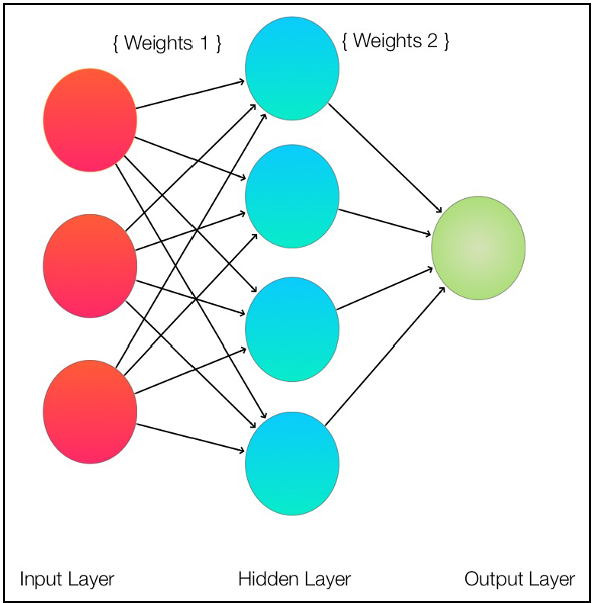
\includegraphics[scale=0.74]{兩層神經網路}
\caption{\Large 兩層神經網路}\label{兩層神經網路}
\end{center}
\end{figure}

 (圖.\ref{兩層神經網路})展示了兩層類神經網路的架構,如圖所示每一層每一個神經元都會連接到下一層全部的神經元,對於每個神經元的連線會給出權重。\\

 神經元是AI系統中使用的軟件模型,其行為或多或少像實際的大腦神經元,模型會使用數字,使一個或另一個神經元對結果有重要的影響,這些數字又稱為權重。\\

 (圖.\ref{兩層神經網路})也展示了輸入層、隱藏層和輸出層,這是最陽春的網路,真正的網路可以更複雜且有更多層次,事實上深度學習命名原則,就是由多層的隱藏層而來,從意義上來說就是增加了類神經網路的深度。\\

 此外,如(圖.\ref{兩層神經網路})所示,是具有過濾層並在​​其中從左到右處理信息,數據輸入的方向只有一個,故被稱為前饋輸入(feed-forward input)。\\

 有了網路架構,就能進一步讓網路學習,神經元網路會接收一個例子並猜測答案,如果答案是錯誤的,它會回溯並修改對神經元施加權重和偏差,並嘗試通過更改某些值來修復錯誤,這樣的行為就被稱為反向傳播(backpropagation)。使用迭代方法進行反複試驗,模擬人們重複的行為,執行經過多時後,最終類神經網路學習會進步並給出更好的答案,訓練時間可以是一天,甚制是一個禮拜,才能完成學習複雜的項目,故每一次的迭代被稱為epoch。\\

 可以看到該神經網絡的輸出僅取決於互連的權重,還取決於神經元本身的偏差,雖然權重會影響啟動函數曲線的陡度,但是偏差會將發生變化的整個曲線,像右或向左,權重和偏差的選擇,決定了單個神經元的預測強度,而訓練神經
網絡使用的輸入數據可以來微調權重和偏差。\\
\subsection{啟動函數}
啟動函數是設計類神經網路的關鍵部分,如果不使用啟動函數,每一層神經元連接到下一層神經元,只會有線性組合,作為輸出,類神經網路便失去了意義,也就是說啟動函數能讓神經元間的連線,產生非線性的組合並作為該層的輸出。\\
以下介紹幾種較為常見的啟動函數及其特性:
\begin{itemize}
%=----------Sigmoid      Function----------=%
\item Sigmoid Function:\\
輸出介於0到1之間,適用於二元分類,方程式具有非線性、可連續微分、並具有固定輸出範圍等特性,並可以讓類神經網路呈現非線性。\\
$$\sigma(x)=\frac{1}{1+e^{-x}}$$
%=----------SigmoidPrime Function----------=%
SigmoidPrime Function是從Sigmoid Function微分得來,以梯度運算的方式,可以減少梯度誤差,但也是造成梯度消失的主要原因,若要改善梯度消失需要搭配優化器使用,方程式如下:\\
$$\sigma^{'}(x)=\sigma(x)[1-\sigma(x)]$$
%=----------Softmax Function----------=%
\item Softmax:\\
Softmax會計算每個事件分布的機率,適用多項目分類、其機率總合為1。以此專案為例,假設擊錘移動有向上移動、向下移動及不移動這三個決策選項,則這三個決策機率值總和為1。\\
$$S(x)=\frac{e^{x_i}}{\sum^k_{j=1}e^{x_i}}$$
%=----------Relu Function----------=%
\item ReLU Function:\\
ReLU Function方程式特性:若輸入值為負值,輸出值為0;若輸入值為正值,輸出則維持該輸入數值。ReLU計算方式簡單、收斂速度快,這是類神經網路最普遍拿來使用的啟動函數,因為可以解決梯度消散的問題,但須注意:起始值若設定到不易被激活範圍或是權重過度所導致權重梯度為0就會造成神經元難以被激活。\\
$$f(x)=max(0,x)$$
$$if , x<0 , f(x)=0$$
$$else f(x)=x$$
%=----------Adam Function----------=%
\item Adam Function\\
結合了 Adagrad 和 RMSprop的優勢,有論文表示,在訓練速度方面有巨大性的提升,但在某些情況下,Adam實際上會找到比隨機梯度下降法更差的解決方法。以下是計算過程:\\
$$g_t=\delta_{\theta}f(\theta)$$
一次矩指數移動均線 :\\
$$m_t =\beta(m_{t-1})+(1-\beta_1)(\nabla{w_t})$$
$$\hat m_t=\frac{m_t}{1-\beta_1^t}$$
二次矩指數移動均線 :\\
$$v_t=\beta_2(v_t-1)+(1-\beta_2)(\nabla{w_t})^2$$
$$\hat{v_t}=\frac{v_t}{1-\beta_2^t}$$
因此,Adam Function:\\
$$\omega_{t-1}=\omega_t-\frac{\eta}{\sqrt{\hat{v_t}-\epsilon}}\hat{m_t}$$
%=----------Mean Squared Error----------=%
\item Mean Squared Error\\
他能告訴你一組點與回歸線接近的程度,透過獲取點與回歸線之距離(這些距離就是誤差)並對它們進行平方來做到這點,而平方是為了消除所有負號,也能讓更大的差異賦予更大的權重。\\
\vspace{8cm}
%(\href{https://www.statisticshowto.com/mean-squared-error/}{\underline{Extracted from here)}}.\\
\begin{figure}
\begin{center}
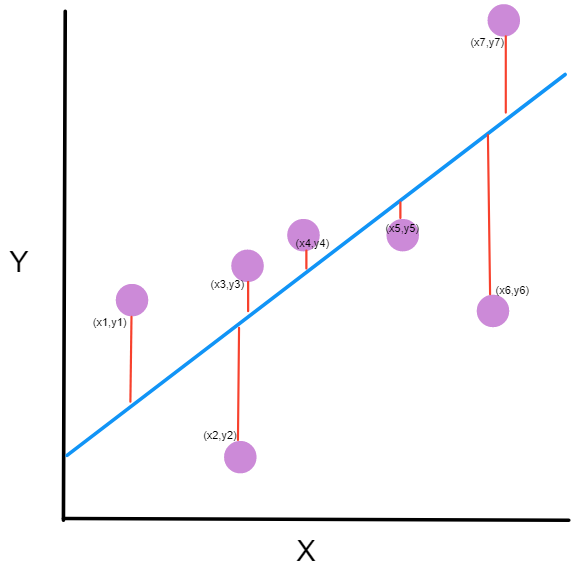
\includegraphics[scale=0.6]{MSE}
\caption{\Large 線性回歸}\label{線性回歸}
\end{center}
\end{figure}
\\
回歸線 :數據點間最小距離的一條線。 \\
n : 數據點的數量\\
$y_i$ :  觀測值\\
$\hat{y_i}$ : 預測值\\
$$MSE=\frac{1}{n} \sum_{i=1}^n(y_i-\overline{y} _i)^2$$\\
\end{itemize}

\subsection{損失函數}
損失函數是類神經網路的最後一塊拼圖,損失函數會將神經網絡的結果與期望的結果進行比較,且必須重複估算模型當前狀態的誤差,就是說該函數可用於估計模型的損失,以便可以更新權重以減少下次評估時的損失,以下將介紹幾種優化的方法:\\

\begin{itemize}
\item Gradient Descent\\
利用梯度的方式尋找最小值的位置,其特色可找到凸面error surface的絕對最小值,在非凸面error surface上找到相對最小值。其缺點是在非凸面error surface要避免被困在次優的局部最小值。
\item Batch gradient descent\\
用批次的方式計算訓練資料,整個資料集計算梯度只更新一次,因此計算和更新時會占用大量記憶體。整體效率較差、速度較緩慢。由 Gradient Descent 延伸出來的算法。其收斂行為與 Gradient Descent 相同。
\item Stochastic gradient descent\\
每次執行時會更新並消除誤差,有頻繁更新和變化大的特性,較不容易困在特定區域。由 Gradient Descent 延伸出來的算法。其收斂行為與 Gradient Descent 相同。
\item Mini-batch gradient descent\\
結合 Batch gradient descent 和 Stochastic gradient descent 的特點:批量計算和頻繁更新,所衍伸的算法。利用小批量的方式頻繁更新,並使收斂更穩定。其缺點:學習率挑選不易、預定義 threshold 無法適應數據集的特徵、對很少發生的特徵無法執行較大的更新、非凸面error surface要避免被困在次優的局部最小值等。
\item Gradient descent optimization algorithms\\
為了改善前面幾種算法而發展出來的優化算法。以下將列出數種優化算法。
\item Momentum\\
在梯度下降法加上動量的概念,會加速收斂到最小值並減少震盪。
\item Nesterov accelerated gradient\\
NAG,有感知能力的 Momentum:在坡度變陡時減速,避免衝過最小值所造成的震盪(為了修正到最小值,來回修正而產生的震盪)。
\item Adagrad\\
其學習率能適應參數:頻繁出現的特徵用較低的學習率,不經常出現的特徵則用較高的學習率,且無須手動調整學習率。其缺點是,學習率會急遽下降,最後會無限小,這算法就不再獲得知識。
\item Adadelta\\
為 Adagrad 的延伸,下降激進程度,學習率從更新規則中淘汰,不需設定預設學習率。
\item RMSprop\\
為了解決 Adagrad 學習率急劇下降的問題,學習率除以梯度平方的RMS,解決學習率無限小的情形。
\item Adam\\
類似 Momentum,更加穩定快速的收斂。
\item AdaMax\\
與 Adam 相似,依靠$(u_t)$ 最大運算。
\item Nadam\\
結合 Adam 和 NAG ,應用先前參數執行兩次更新,一次更新參數一次更新梯度。
\item AMSGrad\\
改善 Adam 算法所導致收斂較差的情況(用指數平均會減少其影響),換用梯度平方最大值來做計算,並移除去偏差的步驟。是否有比 Adam 算法好仍有待觀察。
\item Gradient noise\\[6pt]
有助於訓練特別深且復雜的網絡,noise 可改善不良初始化的網路。
\end{itemize}
\subsection{優化算法}
\newpage
\section{強化學習}
%=----------What is Reinforcement Learning?------------=%
強化學習是通過agent(代理)與已知或未知的環境持續互動,不斷適應與學習,得到的回饋可能是正面,也就是獎賞(reward),如果得到負面,那就是懲罰(punishments)。考慮到agent與環境(environment)互動,進而決定要執行哪個動作,強化學習的學習模式是建立在獎賞與懲罰上。\\
強化學習與其他學習法不一樣的地方在於:不需要事先收集大量數據提供當作學習樣本,而是透過與環境互動,在環境下發生的狀態當作學習的來源。不會像其他機器學習形式的機器人那樣被告知要採取哪些行動,但機器必須發現哪些動作會產生最大的獎勵。\\
由於強化學習是建立在環境上,因此許多參數進行運算,需要大量信息來學習,並根據此採取行動。強化學習的環境是真實世界,可能是2D或3D模擬世界的場景,也可能是建立於遊戲的場景。從某種意義上來說,強化學習的範圍很廣,因為環境的規模可能很大,並且在環境中有多相關因素,影響著彼此。強化學習以獎勵的方式,促使學習結果趨近或達到目標結果。\\
%=----------Faces of Reinforcement Learning---------------=%
強化學習涵蓋範圍:\\

%======需文字補充========%
\begin{figure}[hbt!]
\begin{center}
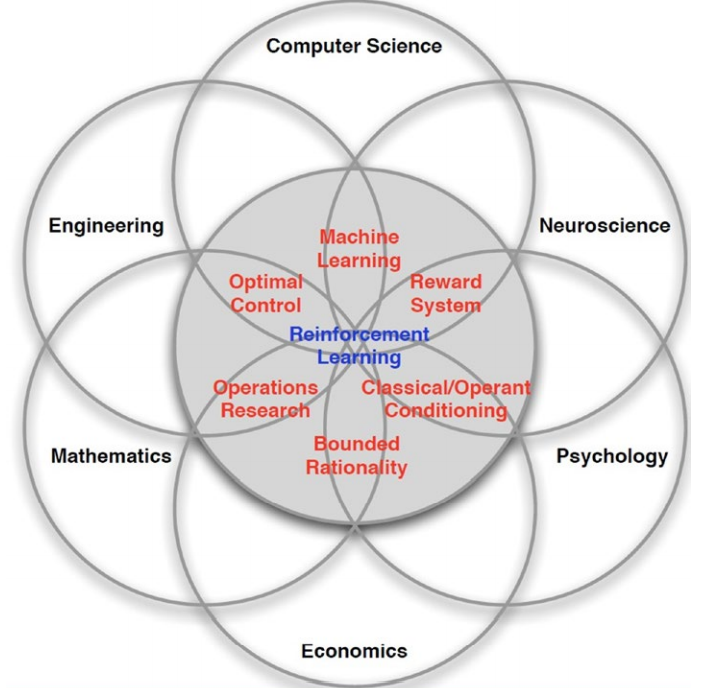
\includegraphics[scale=0.6]{Faces_of_Reinforcement_Learning}
\caption{\Large 文氏圖}
\label{文氏圖}
\end{center}
\end{figure}
%=--------The Flow of Reinforcement Learning------------=%.
強化學習的流程:\\
透過agent與環境間互動而產生狀態和獎勵,由於狀態的轉移,agent會決定接下來執行動作(圖.\ref{RL structur})。\\[12pt]

\begin{figure}[hbt!]
\begin{center}
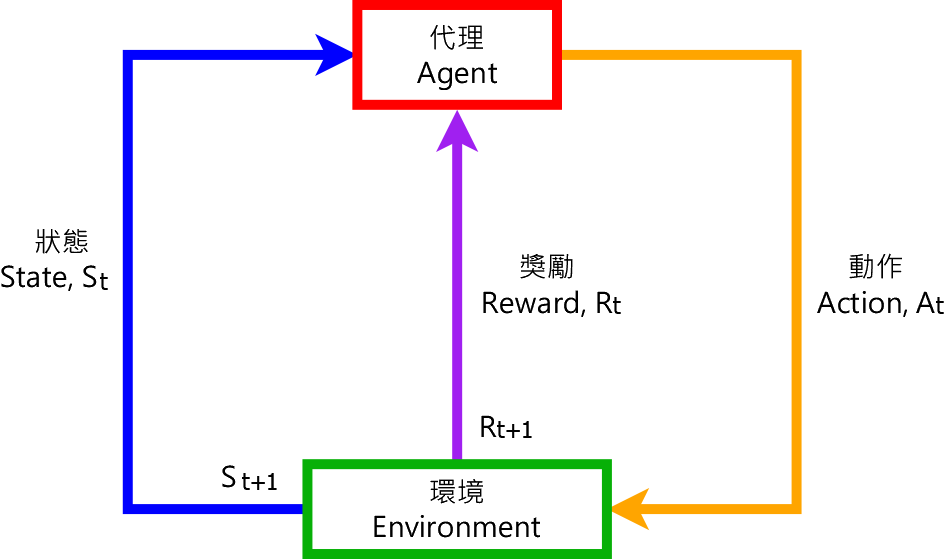
\includegraphics[width=10cm]{The_Flow_of_Reinforcement_Learning}
\caption{\Large RL 架構}
\label{RL structur}
\end{center}
\end{figure}

需要考慮的重點:\\
強化學習的週期是互相聯繫的,分明的溝通是在考慮獎勵的情況下發生的,agent與環境之間存在著獨特的溝通。狀態和動作互相關聯著,並互相影響著彼此:目標或機器人會因動作而造成狀態轉移,狀態的移轉也會影響目標或機器人做出的決策。\\

\begin{figure}[hbt!]
\begin{center}
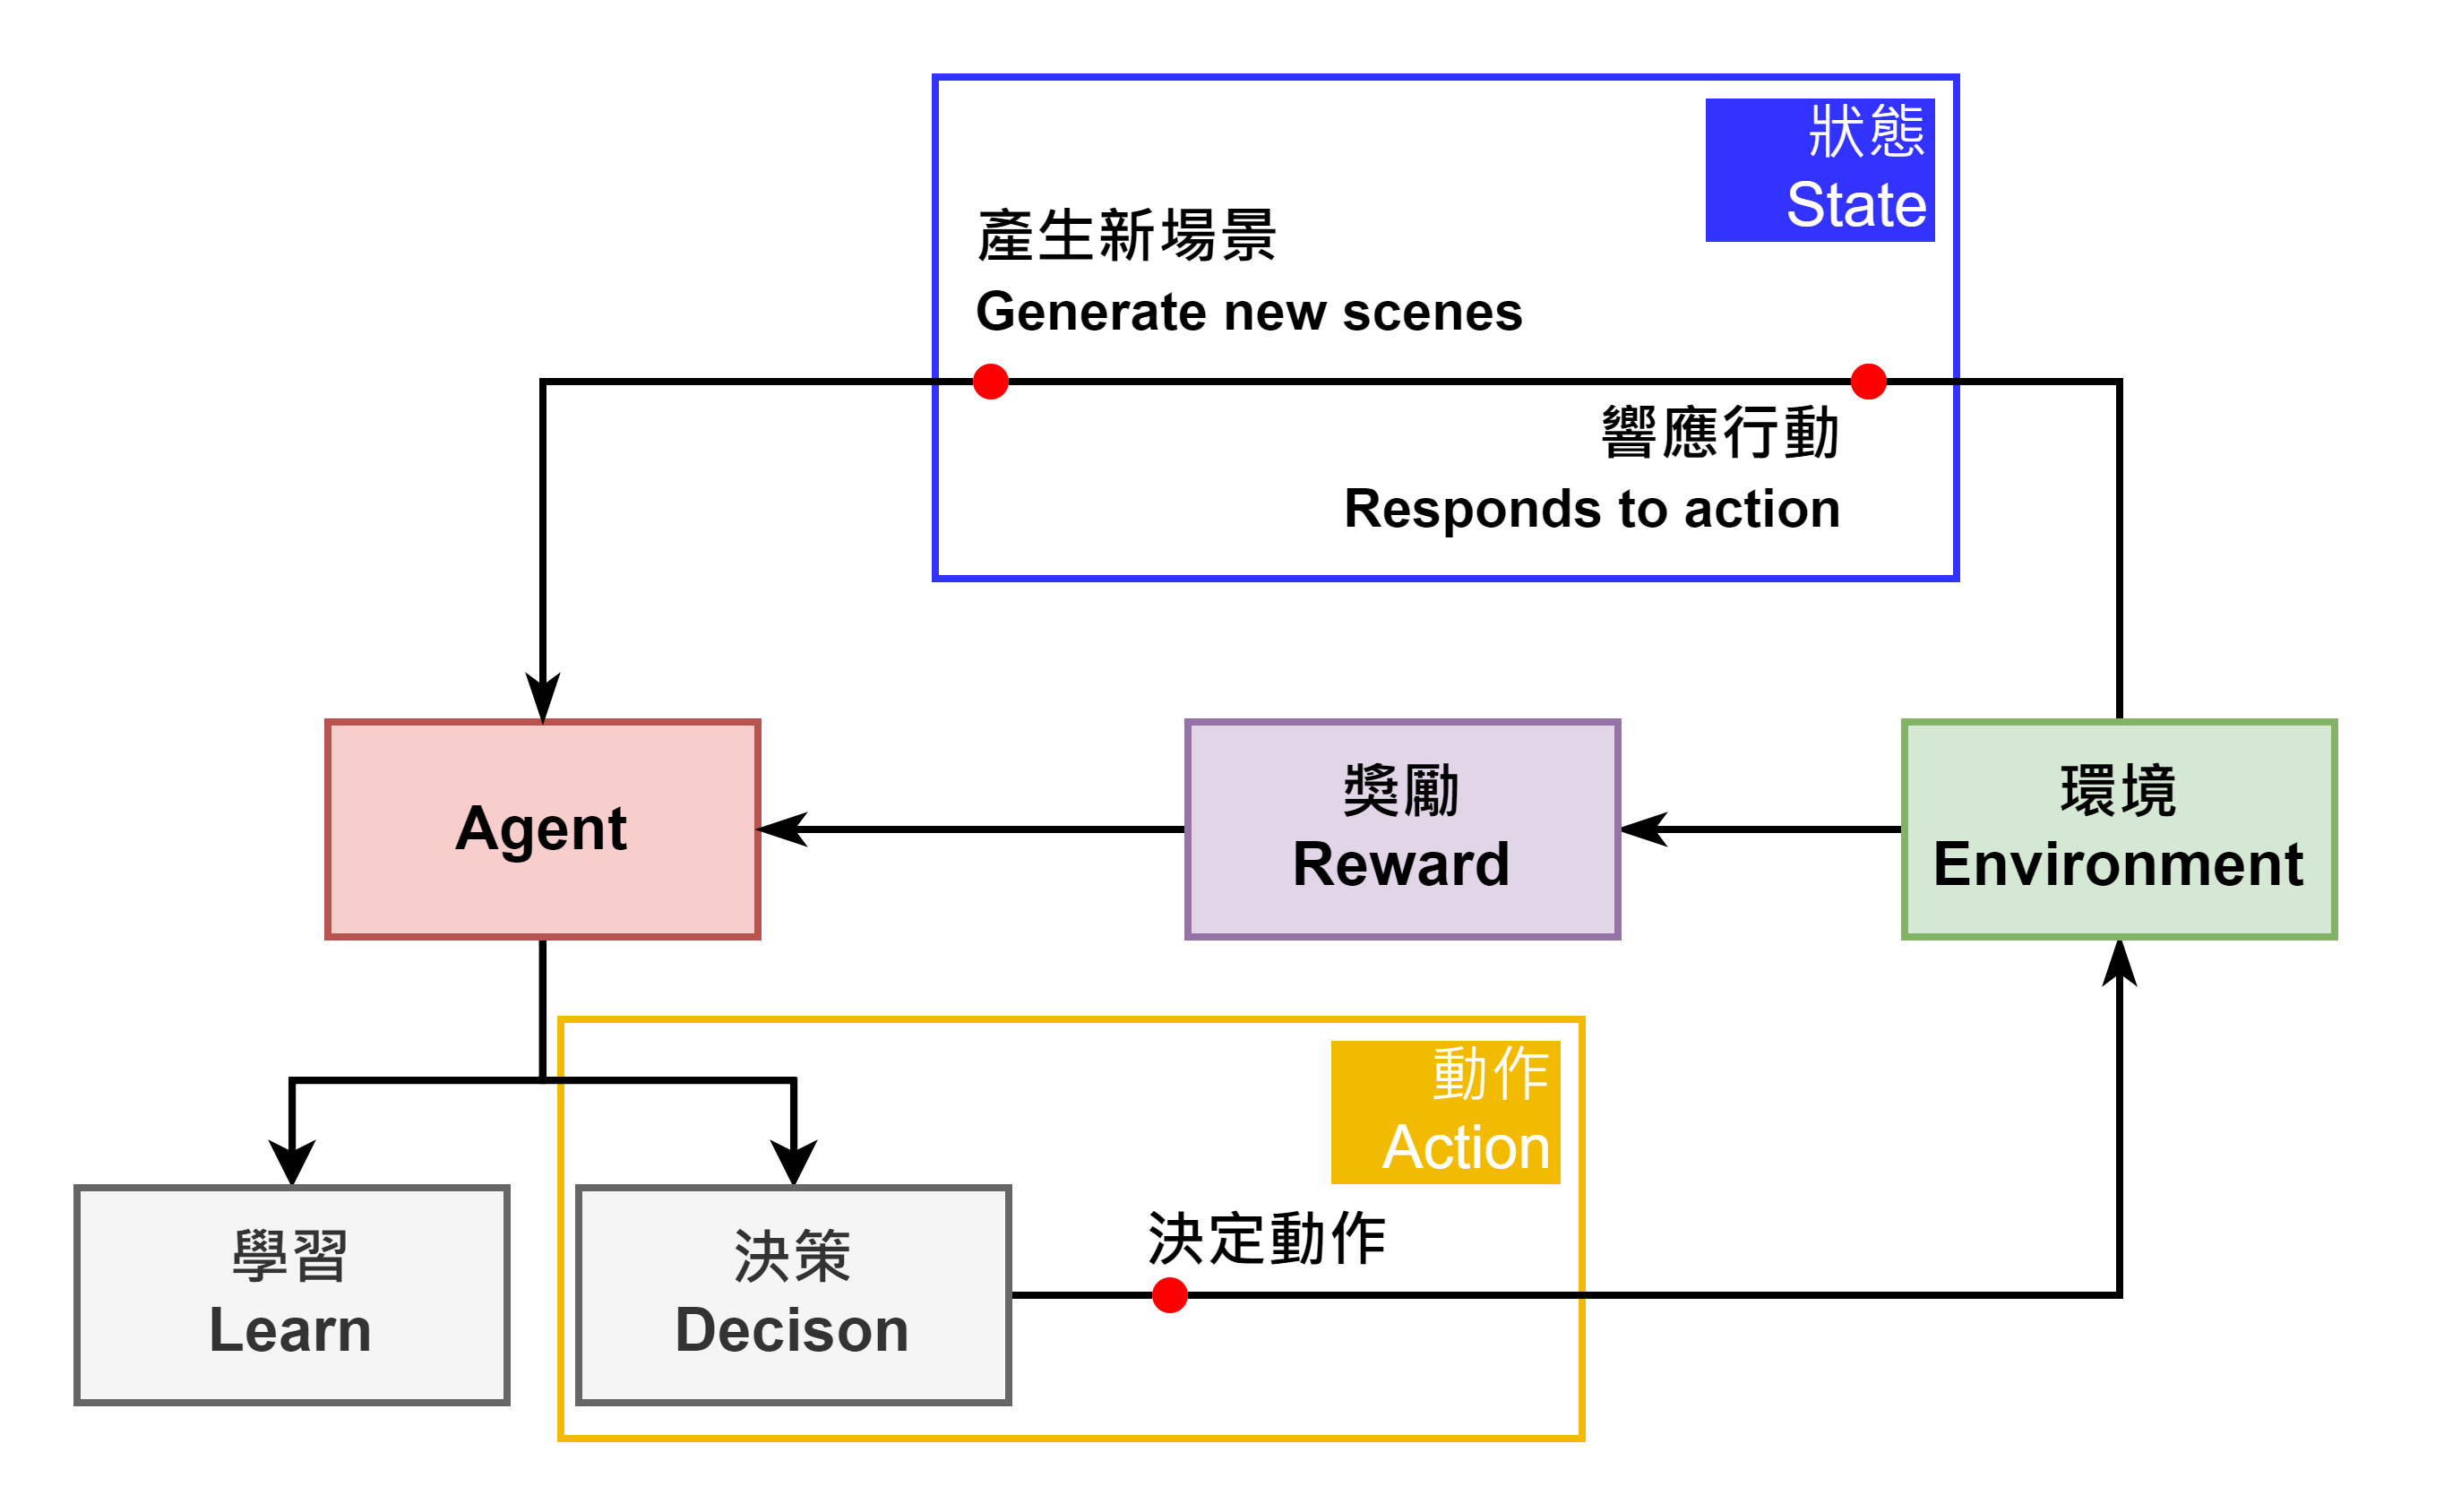
\includegraphics[height=6.3cm]{The_entire_interaction_process}
\caption{\Large 整個互動過程 }
\label{整個互動過程 }
\end{center}
\end{figure}
 如(圖.\ref{The_entire_interaction_process}) agent是決策者,會試圖採取獲得最高大獎勵的行動。當agent開始與環境互動時,他會做出決策,決策所執行的動作會使場景進入下一個狀態,當環境轉變,環境裡的項目也會跟著變動,這些變化被描述為場景,每個步驟中發生的過度都有助於agent更有效地解決強化學習的問題。\\
%=----Different Terms in Reinforcement Learning----------=%
 強化學習中有兩個很重要的常數:$\gamma$和$\lambda$。$\gamma$用於每個狀態轉換,且在每次狀態變化時,都是一個恆定值,$\gamma$會從你將在每個狀態獲得的獎勵類型中,得到資訊。$\gamma$又叫衰減因子,決定未來可獲得的獎勵類型。當狀態改變時為時常數,gamma允許使用者在每個狀態給予不同形式的獎勵(這種狀況下為0,僅與當前狀態有關係),如果注意到長期獎勵值(則為1,獎勵不因得到的先後順序而有所衰減)。\\
 當我們處理時間問題時,通常使用$\lambda$,涉及更多的連續狀態的預測,每種狀態下的$\lambda$值增加,代表算法學習速度很快,適用強化學習時,更快的算法會產生更好的結果。\\
%------------------圖片可共用----------------------%
\iffalse
\begin{figure}[hbt!]
\begin{center}
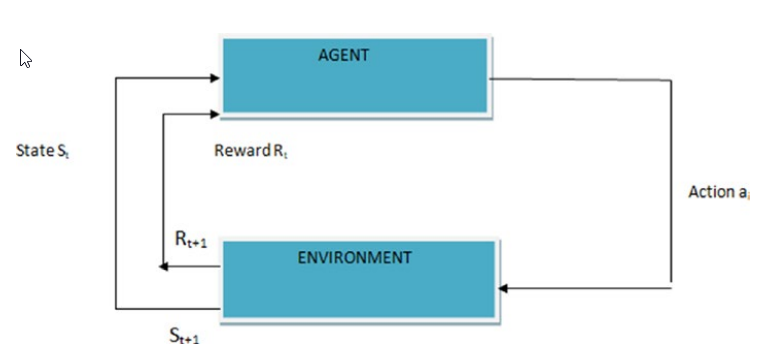
\includegraphics[scale=0.74]{ Reinforcement_Learning_interactions}
\caption{\Large Reinforcement Learning interactions}
\end{center}
\end{figure}
\fi
%=----Interactions with Reinforcement Learning------------=%
強化學習的互動:\\[1pt]
 agent和環境之間的互動會產生獎勵,我們採取行動,從一種狀態轉移到另一種狀態強化學習是一種實現如何將情況映設為行動的方法,從而最大化並找到獲得最高獎勵的方法,機器或機器人不會像其他機器學習形式的機器人那樣被告知要採取哪些行動,但機器必須發現哪些動作會產生最大的獎勵。\\[1pt]
獎勵的目的與運作:\\
 以獎勵的方式誘導機器採取我們所期望的動作或是特定結果。機器會採取最大化獎勵的方式,因此可將目的定為最大獎勵,以吸引機器執行期望做的行為。\\[6pt]
Agents:\\[6pt]
 在強化學習方面,agent可以感知環境時,它可以做出比以往更好的決定。採取的決定就會產生行動且執行的行動必須是最好最佳的。\\[12pt]
\begin{figure}[hbt!]
\begin{center}
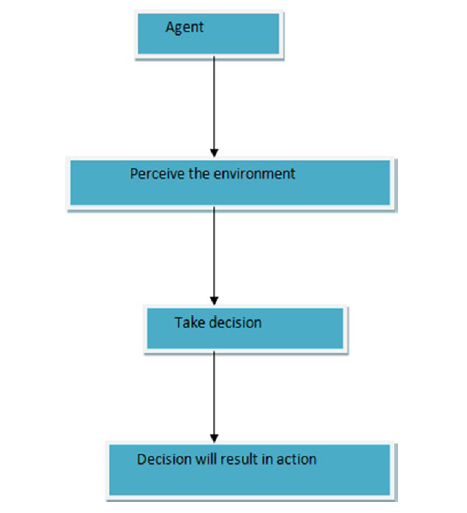
\includegraphics[scale=0.74]{agent}
\caption{\Large agent}
\label{agent}
\end{center}
\end{figure}
%=----Agents------------=%
強化學習的環境\\
\qquad 強化學習中的環境由某些因素組成,會對agent產生影響,agent必須根據環境適應其各種因素,並做出最佳決策,這些環境可以是2D世界或是網格,甚至是3D世界。強化學習的環境具有確定性、可觀察性,可以是離散或是連續的狀態、單個agent或是多個agent\\
\subsection{馬可夫決策}
\begin{itemize}
\item Markov Chain\\
當前決策只會影響下個狀態,當前狀態轉移(action)到其他狀態的機率有所差異。
\item Markov Reward Process\\
action 到指定狀態會獲得獎勵。
$$R(s_t=s) = \mathbb{E}[r_t|s_t = s]$$
$$\gamma \in [0, 1]$$
\begin{itemize}
\item Horizon:
在無限的狀態以有限的狀態表示。
\item Return:
越早做出正確決策獎勵越高。
$$G_t = R_{t+1}+\gamma R_{t+2}+\gamma^2 R_{t+3}+\gamma^3 R_{t+4}+...+\gamma^{T-t-1} R_{T}$$
\item State value function(決策價值):
$$V_t(S) = \mathbb{E}[G_t|s_t = s]$$
$$P(s_{s+1}=s'|s_t=s,a_t=a)$$
\end{itemize}
\item Discount Factor ($\gamma$)
獎勵衰減有幾種作法:第一種,越早做出有獎勵的決策,獎勵越高:第二種,做出有價值的決策$\gamma = 1$,不分決策順序先後;第三種,無用的決策$C = 0$,不會得到獎勵。\\
以Bellman equation的方式描述互動關係狀態:\\
$$V(s) = R(s)+\gamma\sum_{s'\in S}P(s'|s)V(s')$$
\begin{center}
$R(s)$:立即獎勵\\
$\gamma\sum_{s'\in S}P(s'|s)V(s')$:未來獎勵衰減總和
\end{center}
Anaytic solution(分析性解法),MRP的分析性解法:
$$V = (1-\gamma P)^{-1}R$$
Bellman equation及Anaytic solution的方式只適合小的MRP(個數比較少的),矩陣複雜度為$O(N^3)$,N為狀態個數。若要計算大型的MRP會使用疊代法:動態規劃(Dynamic programming)、Temporal-Difference learning和Mote-Carlo evaluation以評估採樣的方式:
$$g = \sum_{i=t}^{H-1}\gamma^{1-t}r_i$$
$$G_t \leftarrow G_t+g,  i \leftarrow i+1$$
$$V_t(s) \leftarrow \frac{G_t}{N}$$
\item Markov Decision Process
\quad 在MRP中加入決策(decision)和動作(action)
\begin{itemize}
\item S:state 狀態
\item A:action 動作
\item P:狀態轉換
$P(s_{s+1}=s'|s_t=s,a_t=a)$
\item R:獎勵,取決於當前狀態和動作會得到相對應的講勵
$$R(s_t=s, a_t=a) = \mathbb{E}[r_t|s_t, a_t=a]$$
\item D:折扣因子(discount factor)
$$\gamma \in [0,1]$$
\end{itemize}
\end{itemize}
馬可夫決策過程以程式方面會以tuple的資料格式表示[程式.\ref{code.MDP code}]:
\label{code.MDP code}
\begin{lstlisting}
 MDP(S, A, P, R, gamma)
\end{lstlisting}

policy(決策):可以是一個決策行為的機率或確定執行的行為,若以數學方程式表示:
$$\pi (a|s) = P(a_t=a|s_t=s)$$
MRP和MDP方程式互相轉換:\\
%=========表格=========%
\begin{center}
\begin{tabular}[c]{ccc}    
%\multicolumn{1}{r}{MRP}
 MRP & $\longleftrightarrow$ & MDP\\
\hline
$P^{\pi}(s's)$ & = & $\sum_{a\in A}\pi (a|s)P(s'|s, a)$\\
$P^{\pi}(s)$ & = & $\sum_{a\in A}\pi (a|s)P(s, a)$\\
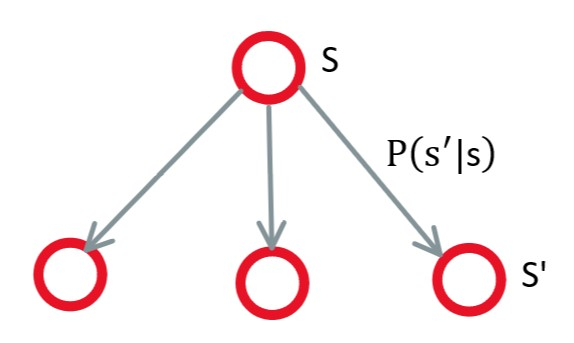
\includegraphics[height=3cm]{MRP}&&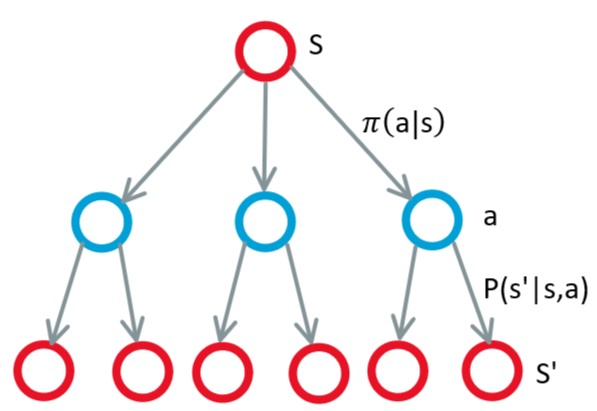
\includegraphics[height=3cm]{MDP}\\
\hline
\end{tabular}
\end{center}

state value function(狀態值方程式)$v^{\pi}(s)$\\
$$v^{\pi}(s) = \mathbb{E}[G_t|s_t=s]$$
$$= \mathbb{E}[R_{t+1}+\gamma v^{\pi}(s_{t+1})|s_t=s]$$
$$= \sum_{a\in A}\pi (a|s)q^{\pi}(s, a)$$
\begin{figure}[hbt!]
\begin{center}
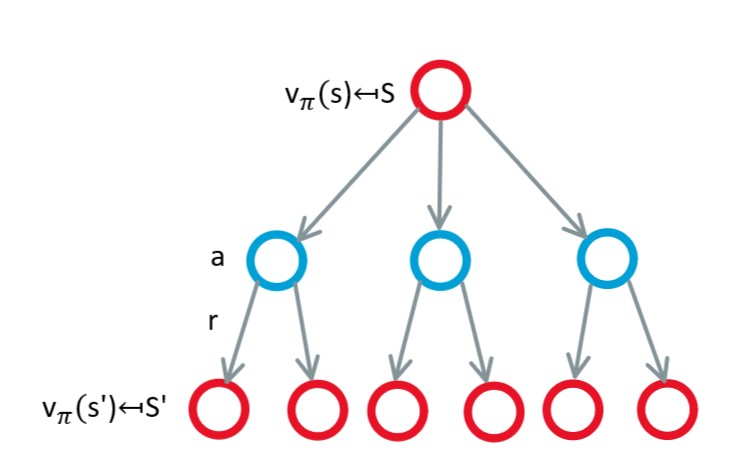
\includegraphics[width=8cm]{s_to _s}
\caption{$v^{\pi}$程序圖}
\label{fig.s_to_s}
\end{center}
\end{figure}
$$v^{\pi}(s) = \sum_{a\in A}\pi (a|s)(R(s, a)+\gamma \sum_{s'\in s}P(s'|s, a)v^{\pi}(s'))$$
state value function(狀態值方程式)$q^{\pi}(s)$
$$v^{\pi}(s) = \mathbb{E}[G_t|s_t=s]$$
$$= \mathbb{E}[R_{t+1}+\gamma v^{\pi}(s_{t+1})|s_t=s]$$
$$= \sum_{a\in A}\pi (a|s)q^{\pi}(s, a)$$
\begin{figure}[hbt!]
\begin{center}
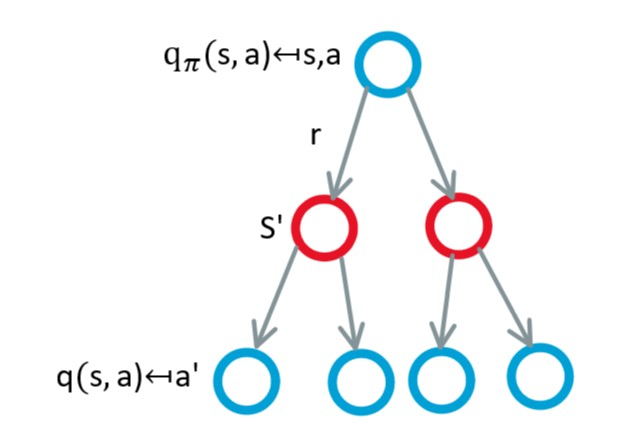
\includegraphics[width=8cm]{Q_pi function}
\caption{$q^{\pi}$程序圖}
\label{fig.q_pi}
\end{center}
\end{figure}
$$q^\pi(s, a)=R(s, a)+\gamma\sum_{s'\in S}P(s'|s, a)\sum_{a'\in A}\pi(a'|s')q^{\pi}(s', a')$$
\newpage
\section{Policy Gradient}
\hspace{-1.5em}$\pi$ : policy\\[5pt]
s : States\\[5pt]
a : Actions\\[5pt]
r : Rewards\\[5pt]
$S_t,A_t,R_t$ : 一個軌跡時間步長't'的State,Action and Reward \\[5pt]
$\gamma$ : Discount Factor;懲罰不確定的未來reward\\[5pt]
$G_t$ : Return;Discounted future reward$G_t = \sum_{k=0}^{\infty} \gamma^k R_{t+k+1}$\\[5pt]
$P(s', r \vert s, a)$ : 伴隨著現在的a和r的state前往下一個state's'的轉移機率矩陣(單階)\\[5pt]
$\pi(a \vert s)$ : 隨機策略(agent的行為策略)\\[5pt]
$\pi_\theta(.)$ : 被$\theta$參數化的策略\\[5pt]
$\mu(s)$ : 確定的策略;我們還使用不同的字母將其標記為$ \ pi(s)$,以提供更好的區分,以便我們可以輕鬆判斷策略是隨機的還是具有確定性的\\[5pt]
$V(s)$ : '狀態值函數'測量state的預期收益(報酬率)\\[5pt]
$V^\pi(s)$ : 根據policy的狀態值函數$V^\pi (s) = \mathbb{E}_{a\sim \pi} [G_t \vert S_t = s]$\\[5pt]
$Q(s, a)$ : '行為值函數'評估一對state and action 的預期收益\\[5pt]
$Q_w(.)$ : 被w參數化的行為值函數\\[5pt]
$Q^\pi(s, a)$ : 根據policy的行為值函數$Q^\pi(s, a) = \mathbb{E}_{a\sim \pi} [G_t \vert S_t = s, A_t = a]$\\[5pt]
$A(s, a)$ : Advantage Function,$A(s, a) = Q(s, a) - V(s)$;像是另一種版本的Q-value;由狀態值為基準降低方差\\[5pt]
參數化 : 待軟體建置於一給定環境時,再依該環境的實際需求填選參數,即可成為適合該環境的軟體。\\[5pt]
強化學習的目標:為agent找到最優的行為策略以獲得最優的報酬\\[5pt]
Policy Gradient的目標:直接建模和優化策略\\[5pt]
reward function的值 : 取決於策略,可應用各種算法optimize$\theta$,已獲得最佳reward\\[5pt]
defined as:\\[5pt]
$$J(\theta) 
= \sum_{s \in \mathcal{S}} d^\pi(s) V^\pi(s) 
= \sum_{s \in \mathcal{S}} d^\pi(s) \sum_{a \in \mathcal{A}} \pi_\theta(a \vert s) Q^\pi(s, a)$$

\subsection{Mokov chain}
stochastic process : 將隨著時間變化的狀態,以數學模式表示\\[5pt]
$+$\\[5pt]
Mokov property : 在目前以及所有過去事件的條件下,任何未來事件發生的機率,和過去的事件不相關僅和目前狀態相關
$d^\pi(s)$ : $\pi_\theta$的Mokov chain 的平穩分布(在$\pi$下的策略狀態分佈) $$d^\pi(s) = \lim_{t \to \infty} P(s_t = s \vert s_0, \pi_\theta)$$
$\ast$ 當策略在其他函數的下標時,將省略 $\pi_\theta$的$\theta$  e.g. $d^\pi(s)$ and $Q^\pi$ should be 
$d^\pi(s)$、$Q^\pi$\\[5pt]
stationary probability for $\pi_\theta$ : 隨著時間進展,結束一個狀態保持不變的機率分布\\
\subsection{為什麼不用value-base而是policy-base}
因為要估計其值得動作和狀態數不勝數,因此在連續空間計算成本太高,$\theta$向$\nabla_\theta J(\theta)$建議方向移動,已找到$\pi\theta$的最佳$\theta$,從而產生最高回報。
\subsection{Proof Policy Gradient Theorem}
計算$\nabla_\theta J(\theta)$depends on 動作選擇和目標選擇行為之後狀態的靜態分布,而導致計算困難。\\[5pt]
Policy gradient theorem : 為目標函式的導數重新建構,使它不涉及$d^\pi(.)$的導數。\\[5pt]
$$\nabla_\theta J(\theta) 
= \nabla_\theta \sum_{s \in \mathcal{S}} d^\pi(s) \sum_{a \in \mathcal{A}} Q^\pi(s, a) \pi_\theta(a \vert s) $$ \\
$$\propto \sum_{s \in \mathcal{S}} d^\pi(s) \sum_{a \in \mathcal{A}} Q^\pi(s, a) \nabla_\theta \pi_\theta(a \vert s)$$
$$\nabla_\theta J(\theta)
= \nabla_\theta V^\pi(s_0)= \sum_{s \in \mathcal{S}} d^\pi(s) \sum_{a \in \mathcal{A}} \pi_\theta(a \vert s) Q^\pi(s, a) \frac{\nabla_\theta \pi_\theta(a \vert s)}{\pi_\theta(a \vert s)}$$
$$=\mathbb{E}_\pi [Q^\pi(s, a) \nabla_\theta \ln \pi_\theta(a \vert s)]  {\text{; Because } (\ln x)' = 1/x}$$
$\ast$ 當狀態和動作分布都遵循策略$\pi_{\theta}$時$\mathbb{E}_{\pi}$表示$\mathbb{E}_{s\sim d\pi,a\sim\pi\theta}$\\[5pt]
Proof $\nabla_\theta J(\theta)
= \nabla_\theta V^\pi(s_0)$ 
$ \nabla_\theta V^\pi(s) $\\[5pt]
=$ \nabla_\theta \Big(\sum_{a \in \mathcal{A}} \pi_\theta(a \vert s)Q^\pi(s, a) \Big)  $\\
$= \sum_{a \in \mathcal{A}} \Big( \nabla_\theta \pi_\theta(a \vert s)Q^\pi(s, a) + \pi_\theta(a \vert s) {\nabla_\theta Q^\pi(s, a)} \Big)  \scriptstyle{\text{; Derivative product rule.}} $\\
$= \sum_{a \in \mathcal{A}} \Big( \nabla_\theta \pi_\theta(a \vert s)Q^\pi(s, a) + \pi_\theta(a \vert s) {\nabla_\theta \sum_{s', r} P(s',r \vert s,a)(r + V^\pi(s'))} \Big)  \scriptstyle{\text{; Extend } Q^\pi \text{ with future state value.}}$ \\
$= \sum_{a \in \mathcal{A}} \Big( \nabla_\theta \pi_\theta(a \vert s)Q^\pi(s, a) + \pi_\theta(a \vert s) {\sum_{s', r} P(s',r \vert s,a) \nabla_\theta V^\pi(s')} \Big)  \scriptstyle{P(s',r \vert s,a) \text{ or } r \text{ is not a func of }\theta}$\\[6pt]
$= \sum_{a \in \mathcal{A}} \Big( \nabla_\theta \pi_\theta(a \vert s)Q^\pi(s, a) + \pi_\theta(a \vert s){\sum_{s'} P(s' \vert s,a) \nabla_\theta V^\pi(s')} \Big)  \scriptstyle{\text{; Because }  P(s' \vert s, a) = \sum_r P(s', r \vert s, a)}$
Let $\phi(s) = \sum_{a \in \mathcal{A}} \nabla_\theta \pi_\theta(a \vert s)Q^\pi(s, a)$ ; 當
K = 1,我們把所有可能動作總結到目標狀態的轉移機率$\rho^\pi(s \to x, k+1) = \sum_{s'} \rho^\pi(s \to s', k) \rho^\pi(s' \to x, 1)$\\[5pt]
$ {\nabla_\theta V^\pi(s)} $\\[5pt]
$= \phi(s) + \sum_a \pi_\theta(a \vert s) \sum_{s'} P(s' \vert s,a) {\nabla_\theta V^\pi(s')}$ \\[5pt]
$= \phi(s) + \sum_{s'} \sum_a \pi_\theta(a \vert s) P(s' \vert s,a) {\nabla_\theta V^\pi(s')}$ \\[5pt]
$=\phi(s) + \sum_{s'} \rho^\pi(s \to s', 1) {\nabla_\theta V^\pi(s')}$ \\[5pt]
$= \phi(s) + \sum_{s'} \rho^\pi(s \to s', 1) {\nabla_\theta V^\pi(s')}$ \\[5pt]
$= \phi(s) + \sum_{s'} \rho^\pi(s \to s', 1){[ \phi(s') + \sum_{s''} \rho^\pi(s' \to s'', 1) \nabla_\theta V^\pi(s'')]}$ \\[5pt]
$= \phi(s) + \sum_{s'} \rho^\pi(s \to s', 1) \phi(s') + \sum_{s''} \rho^\pi(s \to s'', 2){\nabla_\theta V^\pi(s'')} \\
\scriptstyle{\text{ ; Consider }s'\text{ as the middle point for }s \to s''}$\\[5pt]
$= \phi(s) + \sum_{s'} \rho^\pi(s \to s', 1) \phi(s') + \sum_{s''} \rho^\pi(s \to s'', 2)\phi(s'') + \sum_{s'''} \rho^\pi(s \to s''', 3){\nabla_\theta V^\pi(s''')}$ \\[5pt]
$= \dots \scriptstyle{\text{; Repeatedly unrolling the part of }\nabla_\theta V^\pi(.)}$ \\[5pt]
$= \sum_{x\in\mathcal{S}}\sum_{k=0}^\infty \rho^\pi(s \to x, k) \phi(x)$
$\nabla_\theta J(\theta)
= \nabla_\theta V^\pi(s_0)  \scriptstyle{\text{; Starting from a random state } s_0} $\\[5pt]
$= \sum_{s}{\sum_{k=0}^\infty \rho^\pi(s_0 \to s, k)} \phi(s) \scriptstyle{\text{; Let }{\eta(s) = \sum_{k=0}^\infty \rho^\pi(s_0 \to s, k)}} $\\[5pt]
$= \sum_{s}\eta(s) \phi(s) 
= \Big( {\sum_s \eta(s)} \Big)\sum_{s}\frac{\eta(s)}{\sum_s \eta(s)} \phi(s)  
\scriptstyle{\text{; Normalize } \eta(s), s\in\mathcal{S} \text{ to be a probability distribution.}}$\\[5pt]
$\propto \sum_s \frac{\eta(s)}{\sum_s \eta(s)} \phi(s)  \scriptstyle{\sum_s \eta(s)\text{  is a constant}}$ \\[5pt]
$= \sum_s d^\pi(s) \sum_a \nabla_\theta \pi_\theta(a \vert s)Q^\pi(s, a)  \scriptstyle{d^\pi(s) = \frac{\eta(s)}{\sum_s \eta(s)}\text{ is stationary distribution.}}$

$\nabla_\theta J(\theta)
\propto \sum_{s \in \mathcal{S}} d^\pi(s) \sum_{a \in \mathcal{A}} Q^\pi(s, a) \nabla_\theta \pi_\theta(a \vert s) $\\[5pt]
$= \sum_{s \in \mathcal{S}} d^\pi(s) \sum_{a \in \mathcal{A}} \pi_\theta(a \vert s) Q^\pi(s, a) \frac{\nabla_\theta \pi_\theta(a \vert s)}{\pi_\theta(a \vert s)} $\\[5pt]
$= \mathbb{E}_\pi [Q^\pi(s, a) \nabla_\theta \ln \pi_\theta(a \vert s)]  \scriptstyle{\text{; Because } (\ln x)' = 1/x}$
\\[5pt]
\subsection{Policy Gradient Theorem}
Policy Gradient 通過反覆估計梯度來最大化預期的總reward\\[5pt]
$g = \nabla_\theta\mathbb{E}[\sum_{t=0}^\infty r_t]$ ; $g = \mathbb{E}[\sum_{t=0}^\infty\psi_t\nabla_\theta log\pi_\theta(a_t \vert s_t)]$\\[5pt]
\begin{normalsize}{$\psi_t$ may be one of following:}\end{normalsize}
\begin{itemize}
\item $\sum_{t=0}^\infty r$ : total reward of trajectory
\item $\sum_{t^{'}=t}^\infty r^{'}$: reward following action $a_t$
\item $\sum_{t^{'}=t}^\infty r_t^{'}-b(s_t)$: baseline version of previous formula
\item $Q^\pi(s_t,a_t)$ : state-action value function
\item $A^\pi(s_t,a_t)$ : Advantage Function
\item $r_t+V^\pi(s_t+1)-V^\pi(s_t)$ : TD residual
\end{itemize}
The letter formulas use the definitions\\[5pt]
$V^\pi(s_t) = \mathbb{E}_{s_{t}+1:\infty,a_{t}:\infty}[\sum_{l=0}^\infty r_t+l]$\\[5pt]
$Q^\pi(s_t,a_t) = \mathbb{E}_{s_{t}+1:\infty_,a_{t}+1:\infty}[\sum_{l=0}^\infty r_t+l]$\\[5pt]
$A^\pi(s_t,a_t) = Q^\pi(s_t,a_t)-V^\pi(s_t)(Advantage Function)$\\[5pt]
\subsection{Actor Crtic}
原始的policy gradient 沒有偏差,但方差大;所以提出了許多以下算法來減少方差,同時保持偏差不變\\[5pt]
$$g = \mathbb{E}[\sum_{t=0}^\infty\psi_t\nabla_\theta log\pi_\theta(a_t \vert s_t)]$$\\[5pt]
Actor-Critic : 減少原始政策中的梯度方差包括兩個模型\\[5pt]
Critic : 更新值函數參數w,根據算法,它可以是操作值$ Q_w(a \ vert s)$或狀態值$ V_w(s)$ \\[5pt]
Actor : 按照Critic的建議,將策略參數$ \ theta $更新為$ \ pi\_ \ theta(a \ vert s)$\\[5pt]
\begin{Large}
它如何在簡單的行動價值參與者批評中發揮作用:
\end{Large}
\begin{itemize}
\item 隨機的初始化 s,$\theta$,w ;取樣 a $\sim
\pi_\theta(a \vert s)$
\end{itemize}
\begin{itemize}
\item For $t =1 \sim T:$ 
\begin{enumerate}[1]
      \item 取樣 reward $r_t$ $\sim$ $R(s,a)$ 隨後下一階段 $s^{'}$ $\sim$ $P(s^{'}\vert s,a)$ 
      \item 樣本的下一個動作 $a^{'}$ $\sim$ $\pi_\theta(a^{'}\vert s^{'})$
    
       \item 更新 policy 參數 $\theta$ :\\
       $$\theta\leftarrow\theta+\alpha_\theta Q_w(s,a)\nabla_\theta ln\pi_\theta(a\vert s)$$
       \item 計算校正 (TD error)對於時間t的動作值:\\
       $$\delta = r_t + \gamma Q_w(s^{'},a^{'})-Q_w(s,a)$$並使用它來更新操作action - value function:\\
       $$w\leftarrow w+\alpha_w \delta \nabla_w Q_w(s,a) $$
       \item 更新 $a\leftarrow a^{'}$ and $ s \leftarrow s^{'}$ ; 學習率 : $a_\theta$ 和 $a_w$
    \end{enumerate}   
\end{itemize}\newpage
\section{類神經網路中強化學習的應用}
\begin{figure}[hbt!]
\begin{center}
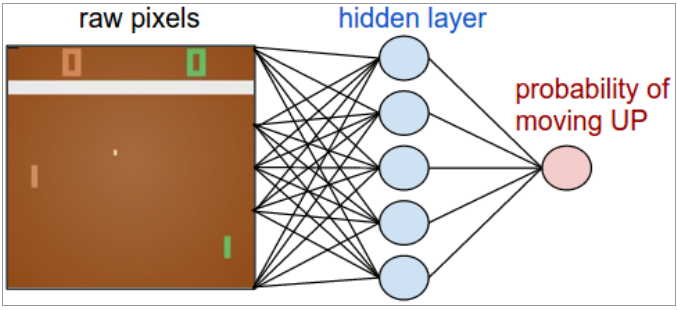
\includegraphics[scale=0.74]{ network}
\caption{實際兩層神經網路}
\end{center}

\end{figure}

 我們將定義一個可以執行我們的玩家(agent)的類神經網路,該網路將獲取遊戲狀態並決定我們應該做什麼(向上移動或向下移動
) 我們使用一個2層神經網路,該網路獲取原始圖像像素(100,800個數字(210*160*3)),並生成一個表示上升概率的數字。 使用隨機策略是標準做法,這意味著我們只會產生向上移動的可能性,每次迭代時,我們都會從該分布中採樣(即扔一枚有偏見的硬幣)已獲得實際移動。\\


\subsection{監督式學習}
\begin{figure}[hbt!]
\begin{center}
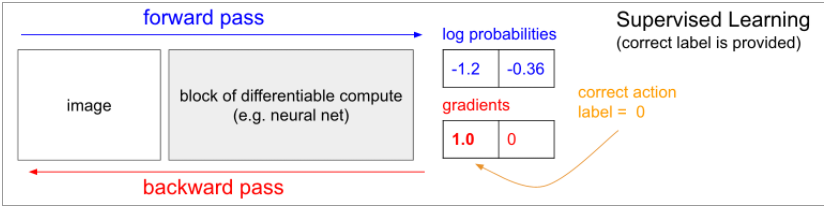
\includegraphics[scale=0.74]{supervising_learning}
\caption{監督式學習}
\end{center}
\end{figure}

 在我們滲入探討 Score Function 解決方案之前,需要簡短介紹有關監督學習的知識,因為正如我們看到的,與我們架構類似,在普通通的監督學習中,我們會將圖像送到網路,並獲得一概率值,例如對於兩個類別的上和下。 這裡顯示的是向上和向下對數概率(-1.2,-0.36),而不是原始機率(在這個情況下,是30$\%$和70$\%$),因為我們總是優化正確標籤的對數概率(這使我們的演算法更好,並等效於優化原始概率,因為對數是單調的),而在監督學習中,我們將可以獲取標籤,例如:\\

我們可能被告知現在正確的做法是向上運動(標籤0),在執行過程中,我們將以上的對數機率輸入1.0的梯度,然後運行backprop來計算梯度向量$Wlogp(y=UP|x)$這個梯度將告訴我們應如何更改百萬個參數中的每個參數,使網路預測往上的可能性更高,例如:網路中的百萬個參數之一可能具有-2.1的梯度,這意味著如果我們將該參數增加一個小的正值(例如0.001),則往上的對數機率將因2.1*0.001而降低(由於負號而減少),如果我們隨後更新了參數,當之後遇到非常相似的圖像時(也就是環境狀況),我們的網路現在更有可能預測往上。\\

\subsection{對數導數技巧}
 機器學習涉及操縱機率。這個機率通常包含normalised-probabilities或 log-probabilities。能加強解決現代機器學習問題的關鍵點,是能夠巧妙的在這兩種型式間交替使用,而對數導數技巧就能夠幫助我們做到這點,也就是運用對數導數的性質。\\
\subsection{為什麼選擇score function 算法}
 多篇論文已經廣泛使用了ATARI遊戲並結合了DQN(它是一種在強化學習算法裡,知名度較高的),事實證明,Q-Learning並不是一個很好的算法,實際上大多數人比較喜歡使用Policy Gradients,包括原始DQN論文的作者,他們在調優後顯示Policy Gradients比Q 首選PG,因為它是端到端的:有一個明確的政策和一種有原則的方法可以直接優化預期的回報。但是礙於時間考量,而選擇了類似PG的算法,也就是score function gradient estimator(取用Andrej Karpathy),從像素開始,通過深度神經網絡使用ATARI遊戲(Pong),並在整個過程結合numpy,作為訓練工具。\\ 
\subsection{Score Functions}
 對數導數技巧的應用規則是基於參數$\theta$梯度的對數函數$p(x:\theta)$,如下:\\
$$\nabla_\theta logp(x:\theta)=\frac{\nabla_\theta p(x:\theta)}{p(x:\theta)}$$\\
$p(x:\theta)$是likelihood ; function參數$\theta$的函數,它提供隨機變量x的概率。在此特例中,$\nabla_\theta logp(x:\theta)$被稱為Score Function,而上述方程式右邊為score ratio(得分比)。\\
score function具有許多有用的屬性:\\

\begin{itemize}
\item 最大概似估計的中央計算。最大概似是機器學習中使用的學習原理之一,用於廣義線性回歸、深度學習、kernel machines、降維和張量分解等,而score出現在這些所有問題中。
\end{itemize}
\begin{itemize}
\item  score的期望值為零。對數導數技巧的第一個用途就是證明這一點。\\
$$\mathbb{E}_{p(x; \theta)}[\nabla_\theta \log p(\mathbf{x}; \theta)] =\mathbb{E}_{p(x; \theta)}\left[\frac{\nabla_\theta p(\mathbf {x}; \theta)}{p(\mathbf{x}; \theta)} \right]$$
$$= \int p(\mathbf {x}; \theta) \frac{\nabla_\theta p(\mathbf {x}; \theta)}{p(\mathbf{x}; \theta)} dx= \nabla_\theta \int p(\mathbf{x}; \theta) dx=\nabla_\theta 1 = 0$$\\
\qquad 在第一行中,我們應用了對數導數技巧,在第二行中,我們交換了差異化和積分的順序,這種特性是我們尋求概率靈活性的類型:  它允許我們從期望值為零的分數中減去任何一項,且此修改不會影響預期得分(控制變量)。
\end{itemize}
\begin{itemize}
\item 得分的方差是Fisher信息,用於確定Cramer-Rao下限。\\
$$\mathbb{V}[\nabla_\theta \log p(\mathbf{x}; \theta)] = \mathcal{I}(\theta) =\mathbb{E}_{p(x; \theta)}[\nabla_\theta \log p(\mathbf{x}; \theta)\nabla_\theta \log p(\mathbf{x}; \theta)^\top]$$\\
我們現在可以從對數概率的梯度躍升為概率的梯度,然後返回,但是真正要解決的其實是計算困難的期望梯度,所以我們可以利用新發現的功能:score function為此問題開發另一個聰明的估計器。
\end{itemize}
\subsection{Score Function Estimators}
我們的問題是計算函數f的期望值的梯度:\\
$$\nabla_\theta \mathbb{E}_{p(z;\theta)}[f(z)] =\nabla_\theta \int p(z; \theta)f(z) dz$$
 這是機器學習中的一項常態性任務,在變數推理中進行後驗計算,在強化學習中進行價值函數和策略學習,在計算金融中進行衍生產品定價以及在運籌學中進行庫存控制等。該梯度很難計算,因為積分通常是未知的,我們計算梯度所依據的參數$\theta$的分佈為$p(z;\theta)$,此外,當函數f不可微時,我們可能想計算該梯度,使用對數導數技巧和得分函數的屬性,我們可以更方便地計算此梯度:\\
$$\nabla_\theta \mathbb{E}_{p(z;\theta)}[f(z)] = \mathbb{E}_{p(z;\theta)}[f(z)\nabla_\theta \log p(z;\theta)]$$
\begin{figure}[hbt!]
\begin{center}
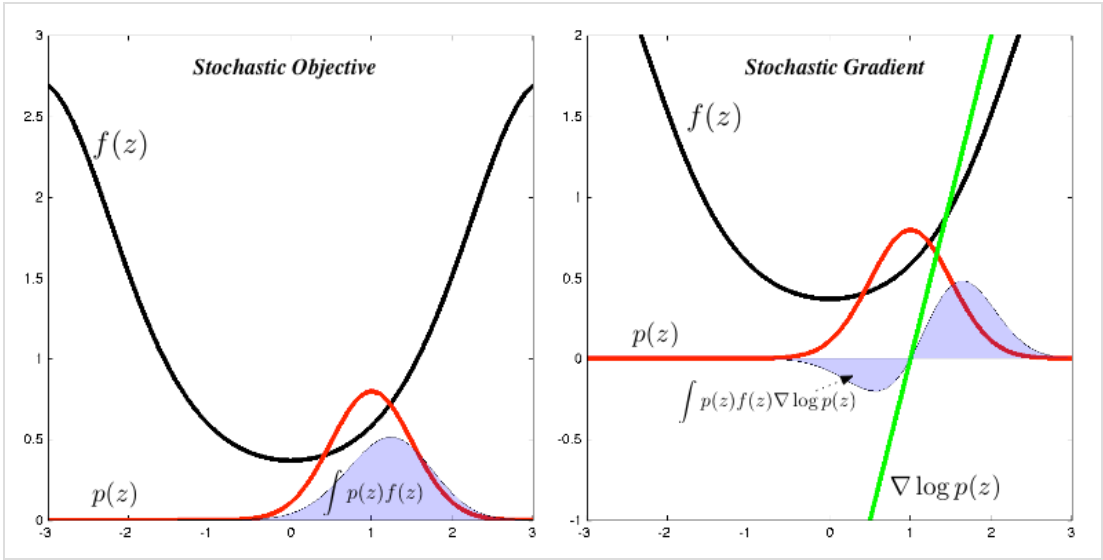
\includegraphics[scale=0.5]{gradient_change}
\caption{gradient change}
\end{center}
\end{figure}
 讓我們導出該表達式,並探討它對我們的優化問題的影響。\\
 為此,我們將使用另一種普遍存在的技巧,一種概率恆等的技巧,在該技巧中,我們將表達式乘以1,該表達式由概率密度除以自身而形成。將特性技巧與對數導數技巧相結合,我們獲得了梯度的得分函數估計量:\\
$$\nabla_\theta \mathbb{E}_{p(z;\theta)}[f(z)]=\int\nabla_\theta p(z;\theta)f(z) dz$$
$$= \int \frac{p(z;\theta)}{p(z;\theta)}\nabla_\theta p(z;\theta)f(z) dz$$
$$=\int p(z;\theta)\nabla_\theta \log p(z;\theta)f(z) dz = \mathbb{E}_{p(z;\theta)}[f(z)\nabla_\theta \log p(z;\theta)]$$
$$=\int p(z;\theta)\nabla_\theta \log p(z;\theta)f(z) dz = \mathbb{E}_{p(z;\theta)}[f(z)\nabla_\theta \log p(z;\theta)]$$
$$\approx \frac{1}{S} \sum_{s=1}^{S}f(z^{(s)})\nabla_\theta \log p(z^{(s)};\theta) \quad z^{(s)}\sim p(z)$$\\
在這四行中發生了很多事情。在第一行中,我們交換了導數和積分。在第二行中,我們應用了概率身份技巧,這使我們能夠形成得分比, 然後使用對數導數技巧,用第三行中對數概率的梯度替換該比率。這在第四行給出了我們所需的隨機估計量,這是由蒙特卡洛計算的,方法是首先從$p(z)$提取樣本,然後計算加權梯度項。.\\

更簡單的描述,我們有一些分佈 $p(x;\theta)$(我使用了速記$ p(x)$來減少混亂),我們可以從中採樣(例如,這可能是高斯)。對於每個樣本,我們還可以評估分數函數f,該函數將樣本作為樣本並給出標量值。該方程式告訴我們,如果我們希望其樣本達到較高的分數(由f判斷),應該如何改變分佈(通過其參數θ),特別是,它看起來像:畫出一些樣本x,評估其分數f(x),並且對於每個x也評估第二項 $\nabla_\theta logp(x;θ)$,那第二項是什麼,它是一個向量-漸變為我們提供了參數空間中的方向,這將導致分配給x的概率增加。換句話說,如果我們要在的方向上微移θ,$\nabla_\theta logp(x;θ)$,我們會看到分配給x的新概率略有增加。如果回顧一下公式,它告訴我們應該朝這個方向發展,並將標量值加到上面$f(x)$。這樣一來,得分較高的樣本將比那些得分較低的樣本“拖拉”更強的概率密度,因此,如果我們要根據p上的幾個樣本進行更新,則概率密度將朝著較高分數的方向移動,從而使得分較高的樣本更有可能出現。\\
\begin{figure}[hbt!]
\begin{center}
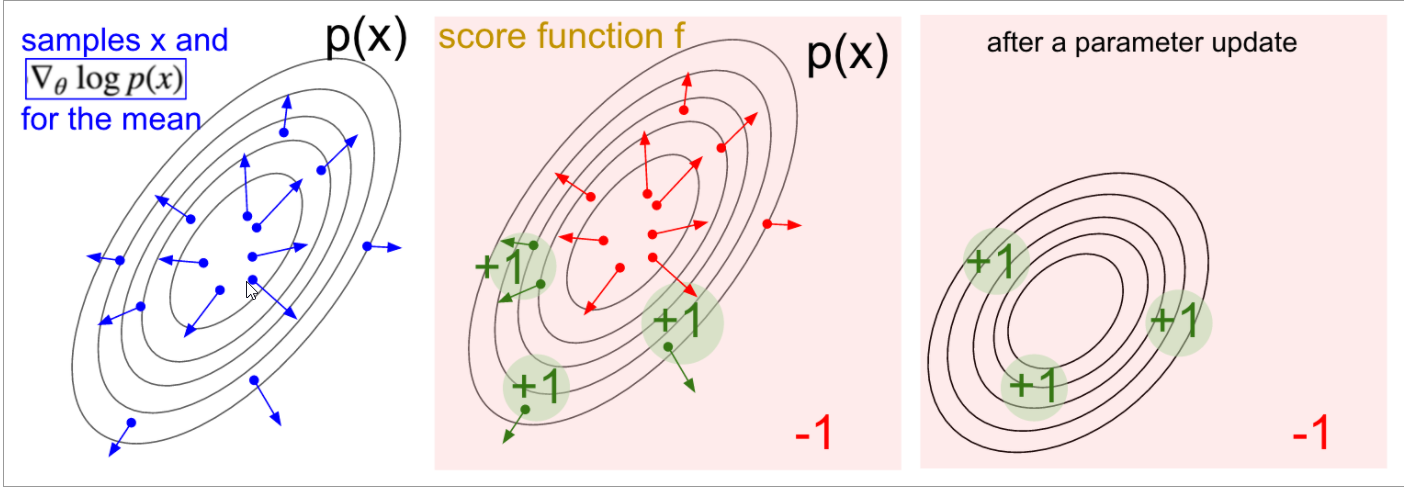
\includegraphics[scale=0.4]{figure}
\caption{梯度變化}
\end{center}
\end{figure}

 Score function gradient estimator的可視化,左:高斯分佈及其中的一些樣本(藍點),在每個藍點上,我們還繪製了相對於高斯平均參數的對數概率的梯度,箭頭指示應微調分佈平均值以增加該樣本概率的方向。中間:某些得分函數的疊加,在某些小區域中除了+1之外,其他所有地方都給出-1(請注意,這可以是任意的,不一定是可微分的標量值函數),箭頭現在採用了顏色區別,因為由於更新中的乘法運算,我們將平均所有綠色箭頭和紅色箭頭的負數。右:更新參數後,綠色箭頭和反向紅色箭頭將我們向左移至底部。現在,根據需要,該分佈中的樣本將具有更高的預期分數。\\
\newpage
\section{比較個方法的特色}
\chapter{訓練環境}
\section{openAI Gym}
 Gym 是用於開發和比較強化學習算法的工具包,他不對agent的結構做任何假設,並且與任何數據計算庫兼容,而可以用來制定強化學習的算法。這個環境具有共享的介面,使我們能用來編寫常規算法,也就能教導agents如何步行到玩遊戲。\\

\section{Pong}
 取自 1977年發行的一款家用遊戲機ATARI 2600中的遊戲,內建於Gym,這是一個橫向的乒乓遊戲,左方是遊玩者,右邊是馬可夫決策的特例,每個邊緣都會給予reward(figue1),目標就是計算再任意階段動作最佳路徑,已獲得rewardd最大值。\\
\section{Pong from pixels}
 左:乒乓球遊戲。右:Pong是Markov決策過程(MDP)的特例:圖,其中每個節點都是特定的遊戲狀態,每個邊緣都是可能的(通常是概率性的)改變,每條邊界都給與獎勵,目標是計算在任何狀態下發揮作用的最佳方式,以最大限度地提高獎勵。\\ 
Pong的遊戲是簡單的強化學習中,很好的例子,在ATARI 2600版本中,我們會控制右邊邊的操縱板(左邊由電腦控制)。遊戲的運行方式如下:我們收到一個圖像幀(一個210x160x3 byte數組(從0到255的整數給出像素值)),然後決定是否要向上或向下移動操縱板(即二進制選擇)。每次選擇之後,遊戲模擬器就會執行動作並給予我們獎勵:如果球超過了對手,則為+1獎勵;如果我們錯過球,則為-1獎勵;否則為0。當然,我們的目標是移動球拍,以便獲得很多獎勵。\\

\newpage
\chapter{模擬環境}
%\renewcommand{\baselinestretch}{10.0} %設定行距
\section{模擬模型}
 在模擬的模型上,延用了學長設計的冰球機,並進行了部分的設計變更,將原本的人機對打更改為機器對打,且因為搭配深度強化學習的訓練,所以將兩邊的擊球器都僅保留X軸向(左右)移動,而冰球則是使用原本設計。多虧了學長們所設計的冰球機模型,讓我們在運作上有問題時可以直接發問,設計變更的地方也可以快速完成。\\
\begin{figure}[hbt!]
\center
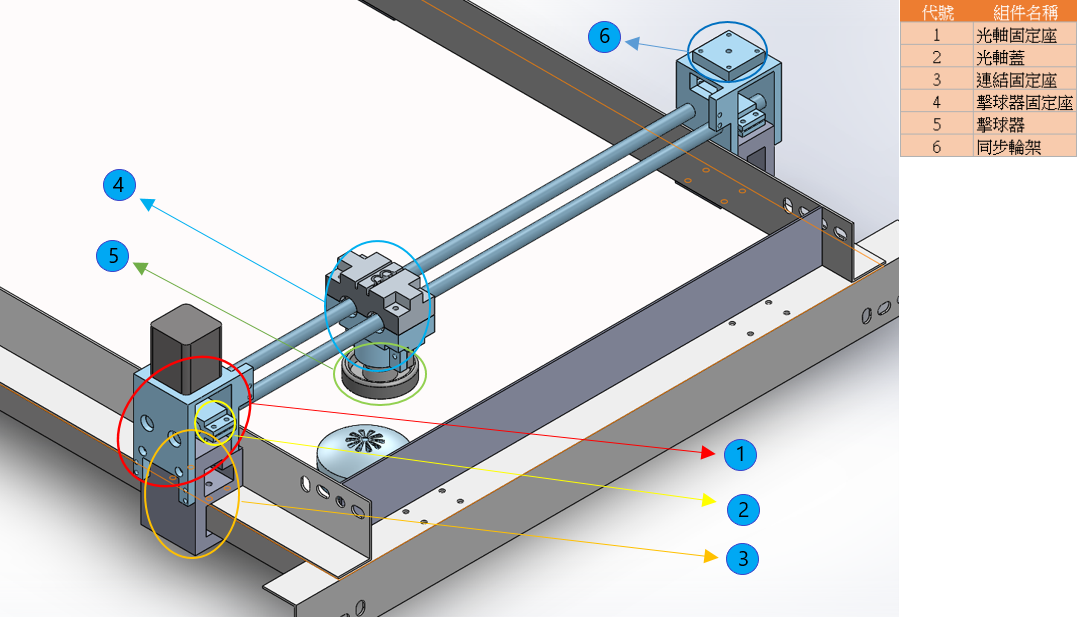
\includegraphics[width=13cm]{model}
\caption{組合圖}
\label{model}
\end{figure}

\qquad 將原本Y軸移動機構移除,並將其改為固定在特定位置上,此固定座設計是取代原本鎖在光軸固定坐上的(圖.\ref{model} 代號 1)Y軸皮帶固定座(圖.\ref{axialseat}),並使光軸固定座可以通過連結固定做鎖固於桌面,如圖.\ref{connectSeat}。\\

\begin{figure}[hbt!]
\center
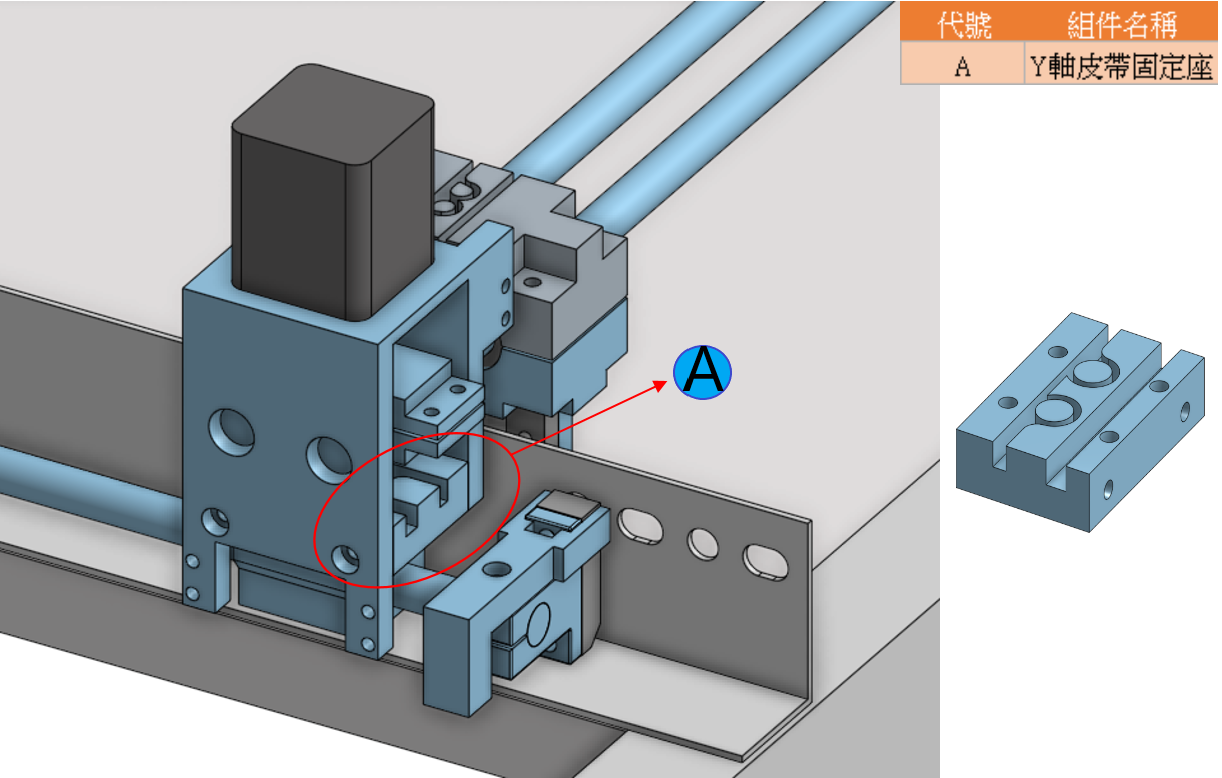
\includegraphics[width=8cm]{axialseat}
\caption{Y軸皮帶固定座}
\label{axialseat}
\end{figure}

\begin{figure}[hbt!]
\center
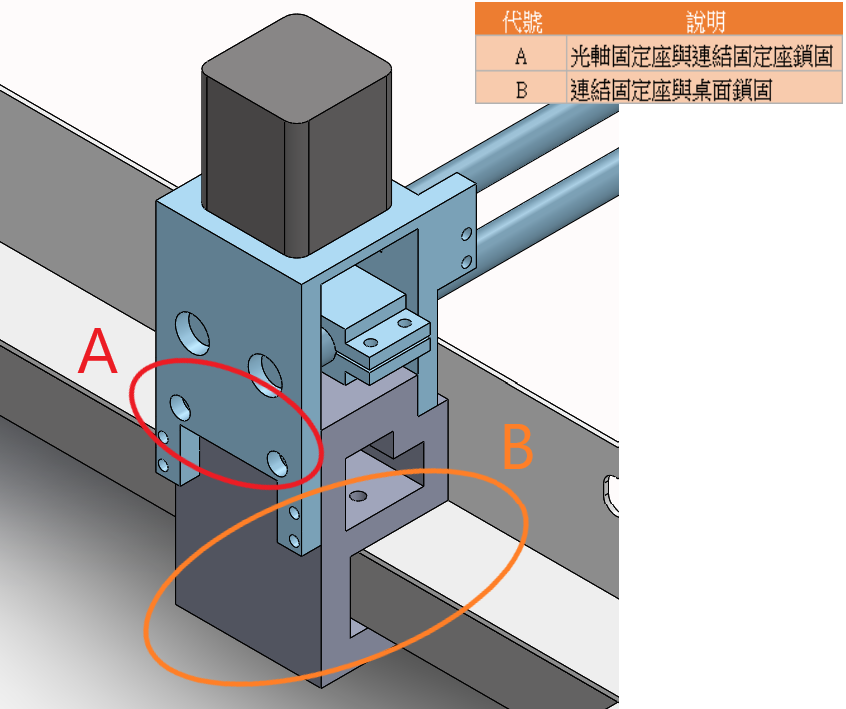
\includegraphics[width=8cm]{connectSeat}
\caption{連結固定座}
\label{connectSeat}
\end{figure}

\newpage
\qquad 分別在擊球器外側保留約冰球直徑1.5倍之區域作為得分判定區,如圖4.4中的紅色區域。\\
\section{CoppeliaSim模擬}
 CoppeliaSim是具有集成開發環境的機器人模擬器,基於分佈式控制體系架構,可以通過嵌入式腳本,插件,ROS或BlueZero節點,RemoteAPI客戶端或自定義解決方案進行模型控制。\\
 \begin{figure}[hbt!]
\center

\includegraphics[width=11cm]{CoppeliaSim}
\caption{CoppeliaSim Logo}
\end{figure}

且CoppeliaSim中,控制器可以用C / C ++、Python、Java、Lua、Matlab或Octave編寫。\\
\subsection{使用原因}
 本專題之最終目標是希望可以在虛擬環境中進行深度強化學習來訓練機器對打,通過虛擬環境中的模擬後,可以更直接地看到深度強化學習訓練的狀況,且因為在虛擬環境中不會有金費的支出,所以可以不斷的重複模擬直到模擬達到最佳的狀態,除此之外CoppeliaSim的虛擬環境更接近真實環境,基於以上原因,所以使用了CoppeliaSim開發。\\
\subsection{RemoteAPI}
 RemoteAPI(Remote Application Programming Interface)是CoppeliaSim API框架的一部分。它允許CoppeliaSim與外部應用程序之間的通訊,是跨平台並支持服務調用和雙向數據流。有兩個不同的版本/框架分別為:Remote API 和The B0-based remote API。\\
\subsection{PyRep}

\subsection{模擬}
\begin{enumerate}

\item 功能說明\\
以下為簡易功能說明:
\begin{figure}[hbt!]
\center
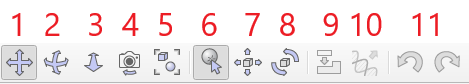
\includegraphics[width=11cm]{toolBar}
\caption{CoppeliaSim 工具列}
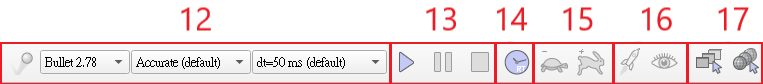
\includegraphics[width=13cm]{toolBar2}
\caption{CoppeliaSim 工具列(續)}
\end{figure}
\begin{table}[hbt!]
\center
\large
\setlength{\tabcolsep}{0.75cm}{
\begin{tabular}{|c|c|c|c|}
\hline  代號 & 功能說明 & 代號 & 功能說明\\
\hline  1 &畫面平移& 10 &複製所有設定\\
\hline  2 &畫面旋轉& 11 &回復/取消回復\\
\hline  3 &畫面縮放&12&模擬設定\\
\hline  4 &畫面視角&13&開始/暫停/停止 模擬\\
\hline  5 &畫面縮放至適當大小&14&即時模擬切換\\
\hline  6 &選取物件&15&模擬速度控制\\
\hline  7 &移動物件&16&線程渲染/視覺化\\
\hline  8 &旋轉物件&17&場景/頁面 選擇\\
\hline  9 &加入/移出 樹狀結構&&\\
\hline 
\end{tabular}}
\caption{功能說明}
\end{table}
\newpage
%\item 模擬執行\\%
\end{enumerate}
\section{影像處理}

\qquad 在影像處理中我們主要使用了Python套件中的OpenCV(全稱:Open Source Computer Vision Library),並搭配其他套件或模組進行了影像處裡,藉此來取得訓練神經網路訓練時所需的資訊。\\
\begin{figure}[hbt!]
\center

\includegraphics[width=10cm]{pythonCVlogo}
\caption{OpenCV 及Python logo}
\end{figure}

\subsection{CoppeliaSim中的Vision sensor(視覺傳感器)}
\qquad CoppeliaSim的視覺傳感器輸出的影像是以每個像素中以RGB三個位元組所組成的,舉例來說:在CoppeliaSim中視覺傳感器取出畫面像素為512*256,則我們會接收到(512*256)像素*3=393,216個資料,是一筆相當大的資料,所以在影像處理上會消耗掉大量的資源。\\

\subsection{影像辨識}
 透過CoppeliaSim中的Vision sensor接收場景影像並輸出後,便可以開始進行影像辨識的處裡\\
\begin{enumerate}
\item RGB與HSV的轉換\\
RGB即光的三原色Red(紅)Green(綠)Blue(藍),HSV則是一種將RGB色彩模型中的點在圓柱坐標系中的表示法,HSV分別表示Hue(色相)、Saturation(飽和度)、Value(明度),而會將RGB轉換為HSV是因為HSV相較於RGB可以更直接的判斷色彩、明暗和鮮豔度對於顏色過濾可以更方便定義出色彩範圍。\\
\begin{figure}[hbt!]
\center
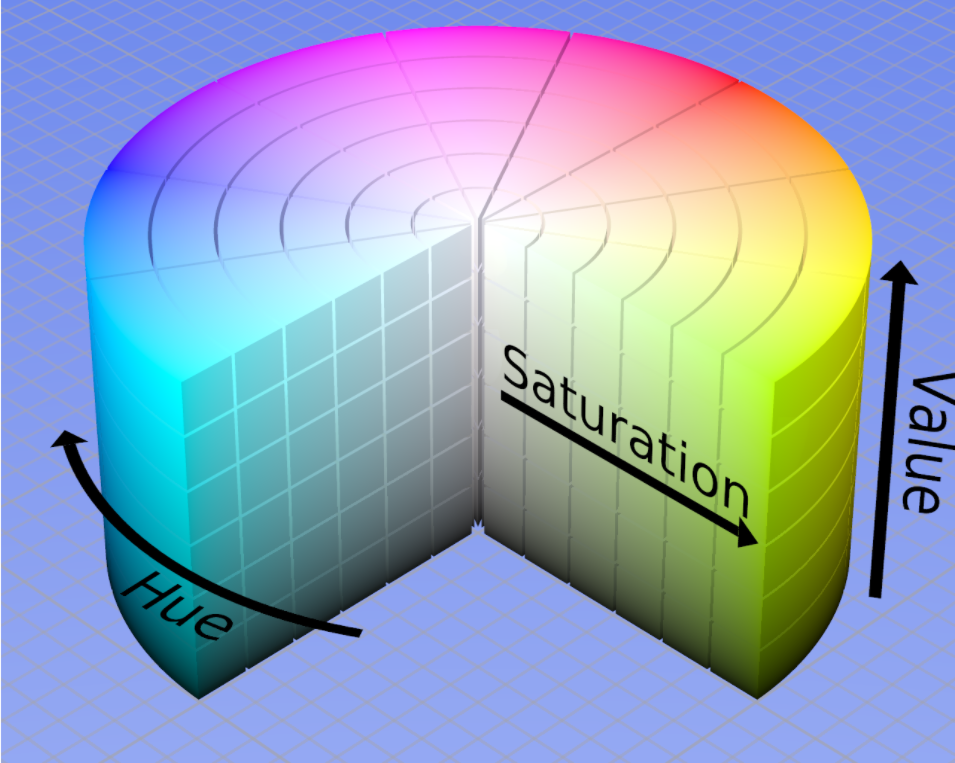
\includegraphics[width=10cm]{HSV}
\caption{HSV色彩空間}
\end{figure}

\item 顏色過濾\\

進行顏色過濾時,需要先定義出過濾顏色的上下限,在開始過濾後僅會保留介於上下界線範圍的影像,而介於上下限範圍之外的影像則會被剃除,如圖.\ref{filter}所示以上限(77,255,255)及下限(35,43,46)為例。\\
\begin{figure}[hbt!]
\center
\begin{minipage}[t]{0.48\textwidth}
\center
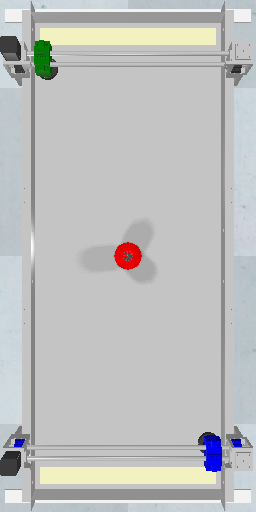
\includegraphics[width=6cm]{origin}
\caption{場景原圖}
\label{origin}
\end{minipage}
\begin{minipage}[t]{0.48\textwidth}
\center
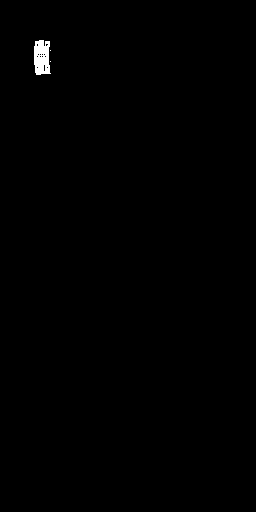
\includegraphics[width=6cm]{filter}
\caption{顏色過濾後的場景}
\label{filter}
\end{minipage}
\end{figure}


%\item 雜訊去除\\
%為了避免環境因素干擾,使影像產生雜訊並影響了影像辨識度,所以在雜訊的去除也是很重要的,

\end{enumerate}

\newpage
\chapter{伺服器}
 此專題採用 Ubuntu 20.04 版本作為我們的架設所使用作業系統,由於 Ubuntu 功能尤為繁多,以下說明重點只著重在專題製作所用到功能上。\\
 
 Ubuntu 作業系統是 Linux 系統的一個發行版,目前免費且開源,Ubuntu 基於 Debian發行版和 GNOME 桌面環境,其目標在於為一般使用者提供一個最新、穩定又主要以自由軟體建構而成的作業系統。\\
 
 其開發目的是為了使個人電腦變得簡單易用,它與其他基於 Debian 所發行的 Linux 版本更加接近 Debian 的開發理念,它主要使用自由、開源的軟體,而其他則帶很多閉源的軟體。\\
\section{Ubuntu 環境配置}
 在一開始會先使用套件管理系統 apt 指令去下載 Xorg , fluxbox , lxde 套件。Xorg 是 Ubuntu 操作系統的一個顯示服務器軟件包,它在被導入 Ubuntu 操作系統後會載入一系列的文件或軟件,這些都是跟顯示卡驅動,圖形環境庫相關的一些文件、軟件。Gnome ,kde,包括我們使用的 lxde 也需要 xorg 才能實現。而 Lxde 它的全名是 Lightweight X11 Desktop Environment ,是自由軟體桌面環境,其優點在於提供了輕量而快速的桌面環境,它比較重視實用、輕巧,除此之外它還可以在 Linux 平台執行。\\
 
 之後需選擇 display manager ( 顯示管理器 )的種類 ,Display manager 是操作系統 Ubuntu 的組件,其中登錄的動作即為 Display manager 負責。該操作系統中常見的類型有 gdm ,gdm3 , lightdm ,kdm ...。各類型的 Display manager 功能其實大同小異,差別在於外觀、操作、格式、複雜度和使用者感受等,可依使用者需求變更 ( 有些較為輕量,適合比較低階的運行器 )。選擇其中一個後繼續,之後可以切換更動 。\\

 再來是模組的導入,此處同樣用 apt 指令安裝 : Pip , uwsgi , Nginx  , 以及 Git 。如果要從 Ubuntu 系統上安裝軟體,其中一種方式是 " pip "。「pip 」是 " pip Installs Packages " 的縮寫,是一個用命令列作為基礎的套件管理系統,可以用它來安裝 python 的應用程式。而使用 Git 是因為在備份資料時, 可幫助使用者有效管理原始碼,而 github 就是由 Git 伺服器和網頁介面組成,用來當作放置原始碼的倉庫。\\
 
 另外 Nginx 和 uwsgi 是為拿來配合把 python 程式應用在網路上實現,並且把想要的結果使其能在網路實時觀看操控結果之反饋。\\
\section{Oracle VM VirtualBox 介紹}
 假使建構虛擬環境時需要在同一主機使用不同電腦作業系統環境,則可使用「虛擬機器工作站」— Oracle VM VirtualBox 。\\

 選擇 Oracle VM VirtualBox    是為了因應當要使用不同作業系統 ( 比如本機與虛擬環境不同作業系統  ) 且不想與其資料存放時共用一個硬碟 ( 無多餘硬碟 , 不想硬碟之間有資料重疊 ... ) 時,即可使用其軟體做練習,降低操作失誤帶來的成本,而此軟體目前為免費,並隨時會更新,另外其特色有 :\\  
\begin{itemize}


\item 只要自備作業系統 ( 光碟片 , ISO映像檔 ) ,即可在啟動 Oracle VM VirtualBox  後直接開啟要操作的執行檔 ( 作業系統 ),不必再把主機本身重新關機,當然開啟多個作業系統之間也有共通性,可直接從視窗A做網路、檔案分享、複製貼上等動作到視窗B。\\
\item 除了作業系統裡面的執行,還可在其中練習磁碟分割、格式化以及 BIOS 啟動等 ( 但是未支援USB啟動 ) 。\\
\item 空間的佔用上並不是真實佔用空間,而是依據使用者的操作而變化 ( 使用者用多少就是多少 )。相對的,使用者雖然一開始設定該虛擬電腦的記憶體大小與硬碟空間是實時依據操作者決定,但終究還是佔掉電腦效能,所以 VirtualBox 的效能還是依據電腦本身的硬體配備。為了配置網路,首先在 : 
\begin{enumerate}
\item File / Preferences / Network  位置,新增一個或右鍵點擊現有的網路設定,填入該電腦網路設定 。
\item Settings / Network / Adapter 1 / Attached to :  該位置改成  Bridged Adapter
\end{enumerate}
\qquad 此處配置之比較 ( 取常用例子 ):NAT , Bridged , Internal , Host-only
\item NAT : 最為基本之設定,主要讓該虛擬主機可連上網,但在與其他網路使用者互動時找不到該虛擬主機網路位址,外部網路也無法偵測,虛擬主機所有的網路請求都會把該來源視為宿主機的。
\item Host-only : 虛擬主機被分配到一個網址,但是還是只有虛擬主機運行的環境可訪問該網路位址
\item Internal : 此種設定主要為虛擬主機彼此間的連線,它可向外部提供資料,但反之則不行。
\item Bridged : 在與其宿主機的網卡設定橋接與設定好外部網路位址後,可被外部網路訪問。
\end{itemize}
\newpage
\section{Web server}
 Nginx 是提供 web 相關服務的伺服器 ( Web server ),除了是高效能的 HTTP ( HTTPS ) 服務器外,還可處理靜態資源 , 負載平衡 , 代理等工作。代理工作為根據不同域名轉發到 Application Server 的不同 port 上去處理 ,其中又分正向和反向,正向代理為 clinet 端發送 request 經由 porxy server 再到目標網站,反向則反之。正向代理操作中 server 只知道 proxy server  給他 request , 不知道 client 是誰,而相同地反向代理則是 client 只知道 proxy server 給他 responses , 不知道 server 是誰。正向代理隐藏真實 Client,反向代理隱藏真實 Server。另外在高流量的狀況下,需要多個 Application Server 來分擔流量,負載平衡就是負責 request 的分發,決定 request 要被分到哪一個 Application Server 處理 。而關於處理靜態資源 ,Nginx 與 Apache 等 Web Server 處理靜態資源的能力是遠遠高於 Application Server 的。\\
 \begin{figure}[hbt!]
\begin{center}
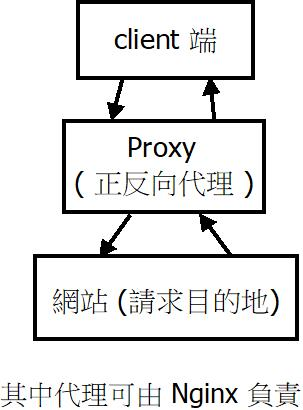
\includegraphics[scale=0.74]{clientProxy}
\caption{\Large clientProxy}\label{clientProxy}
\end{center}
\end{figure}

\section{Nginx}
 網路設定:\\
 首先要修改網路設定檔 ,而其設定檔放在 /etc / netplan 目錄下的 yaml 檔 。其中需更改的設定 :
\begin{enumerate}
\item addresses: 為靜態 IP,可以是IPV4或IPV6。
\item gateway: 即為該電腦之閘道器。
\item nameservers: 該電腦之DNS服務器。
\end{enumerate}

 WSGI ( Python Web Server GateWay Interface ) 為一種用在 Python 語言上的規範,用來規範 Web Server 與 Web Application 之間如何溝通。而 uWSGI 同為實現了 WSGI ,uwsgi , http 協議等的 Web server , 通常用於接收前端伺服器轉發的動態請求並轉發給 Web Application 。前者可以使用 Nginx 提供的 https 協定,且同上表述中 Nginx 的靜態資源處理能力較佳所以也能將靜態資源轉給其處理。\\
 
Nginx 的主要設定檔 nginx.conf 可藉由 include 指令添加其他 nginx 設定檔的設定去擴增不同域名的設定,常見的設定有 :
\begin{enumerate}
\item 預設:
\begin{lstlisting}[caption=nginx預設]
  reciveAPP {
    server localhost:5000;
    server localhost:5001;
}

server {
    listen 80;
    listen [::]:80;
    server_name SERVER_IP;
    root /home/hostname;

    location / {
            uwsgi_pass http://api/;
            include uwsgi_params;
    }
\end{lstlisting}

\newpage
\item 負載平衡LoadBalance:
\begin{lstlisting}[caption=load balance設定]
  reciveAPP {
        ip_hash;
        server localhost:5000;
        server localhost:5001;
}

server {
    listen 80;
    listen [::]:80;
    server_name SERVER_IP;
    root /home/ryan;

    location / {
            uwsgi_pass 127.0.0.1:8000;
            include uwsgi_params;
    }
}
\end{lstlisting}
\end{enumerate}

 reciveAPP 定義了將 request proxy 過去的應用,例子中 server localhost 語法代表可以請求 proxy 到分別監聽 5000 與 5001 port 的兩個應用,同時這個 block 可達到 load balancer 負載平衡的功能 。\\
 
 server 這個 block 則是定義了proxy server的相關設定,包括要監聽的port( listen 80 為監聽所有 IPV4位址, listen [::]80 則為監聽所有 IPV6位址 )、規定哪些 domain 或 ip 的 request 會被 nginx server 處理(server\_ name)。\\
 location 像是 路由 (routing) 的概念,設定不同的 path 要對應到怎麼樣的設定。location 中則是指對不同路徑的處理。\\
 
\begin{enumerate}
\item location:
\begin{lstlisting}[caption=location設定]
  location / #匹配所有目錄

  location /static #匹配所有 /static 的開頭目錄
\end{lstlisting}
\end{enumerate}

 要達到 load balancer 透過一開始介紹的 upstream block 就可以達成,在上面的例子中,來自某個 domain 80 port 會被分配到 port 5000 或 port 5001 兩個應用中,達成用兩個應用去分擔 request 的負載平衡器。\\
 
 負載平衡裡的負載規則  ( ip\_hash ) 某個 request 要被導倒哪個應用去處理有不同規則,每個規則都有各自適合使用時機,以下簡單介紹幾個常見的規則:\\
 
\begin{enumerate}
\item round-robin:(預設)輪詢方式: 也就是將請求輪流按照順序分配給每一個 server。假設所有伺服器的處理效能都相同,不關心每臺伺服器的當前連線數和響應速度。適合於伺服器組中的所有伺服器都有相同的軟硬體配置並且平均伺服器請求相對均衡的情況。
不過也有另外一種可以設定權重的 Weight Round Robin (加權輪詢方式),可以設定不同 server 的權重,例如以下範例:
\begin{lstlisting}[caption=設定不同 server 的權重]
  upstream myweb {
    server web1.dtask.idv.tw weight=3;
    server web2.dtask.idv.tw weight=2;
}
\end{lstlisting}
\item least-connected 最少連線: 顧名思義為連線進來時會把 Request 導向連線數較少的 Server。
\item IP-hash 依據 Client IP 來分配到不同台 Server: 通過一個雜湊(Hash)函式將一個 IP 地址對映到一臺伺服器。先根據請求的目標 IP 地址,作為雜湊鍵(Hash Key)從靜態分配的散列表找出對應的伺服器。除非斷線或 IP變動,否則同個 IP 的請求都會導入到同一個 server。
\end{enumerate}
  uWSGI設定(uwsgi\_ini ):\\
 \begin{enumerate} 
 \item wsgi-file : 主要運行的 py 檔案
 \item http , socket , http-socket : 端口設定,假使有使用到 前端服務器 ( 如Nginx ) 時,不能用 http 設定,因 uwsgi 協議為 HTTP,而 Nginx 使用傳輸協議為 TCP,兩者不能互通。
 \begin{lstlisting}[caption=簡易uwsgi指令啟動]
  uwsgi --http : 9000 --wsgi-file APP.py 
\end{lstlisting}
 \item processes , threads : 工作序, processes 為進程 ,threads 為線程 , 下方設定為每條近程有兩條線程 。
 \begin{lstlisting}[caption=加入工作程序uwsgi指令啟動]
  uwsgi --http : 9000 --wsgi-file APP.py --processes 4 --threads 2
\end{lstlisting}
\item chdir : 此項是為了正確的加載模組 / 檔案 \\

整體快速配置 ( 這裡儲存成一個  .ini 文件,其他還有YAML , JSON , XML 格式等 )  :
\begin{lstlisting}[caption=將uwsgi指令啟動動作設定成一個啟動檔]
  [uwsgi]
socket = :9000
processes = 4
threads = 2
chdir = location/to
wsgi-file = location/to/file
\end{lstlisting}
此項還可加上 status :  此項為查看 uWSGI 內部的輸出數據\\
\begin{lstlisting}[caption=status]
  -- status 127.0.0.1:9001
\end{lstlisting}
實現之通訊流程 
\begin{lstlisting}[caption=client端與Flask應用]
  client server  < - > web server < - > ( socket ) < - > uWSGI < - > flask 
\end{lstlisting}
\begin{figure}[hbt!]
\begin{center}
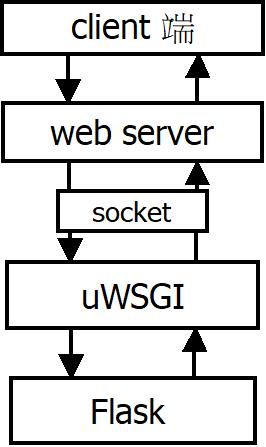
\includegraphics[scale=0.74]{clientToflask}
\caption{\Large clientToflask}\label{clientToflask}
\end{center}
\end{figure}
 \end{enumerate}
\section{Flask}
 
 如同以上所述,建立 Flask 框架的同時需選擇反向代理伺服器 ( 這裡我們選擇了 Nginx ) 來負責網頁請求和結果的回覆,同時還需要一個實現  WSGI 通信協議的伺服器 ( 我們選擇了 uWSGI ) 來負責接收代理伺服器的請求後轉發 Flask 及 接收 Flask 訊息轉發回去 ( 代理伺服器 )。\\
 
\begin{figure}[hbt!]
\begin{center}
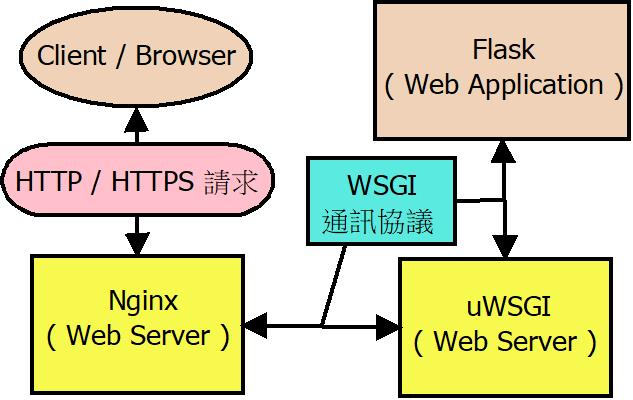
\includegraphics[scale=0.74]{total}
\caption{\Large total}\label{total}
\end{center}
\end{figure}

\chapter{機器學習的訓練與模擬控制結果}
\section{訓練模型的選用}
 利用Gym的環境訓練機器學習,以測試學習率、神經網路隱藏層的神經元個數、機器學習的啟動函數類型、訓練時影像大小等幾項參數與訓結果之間的關聯性,選用pyhton語言進行配置。剛開始我們運用pygame模組來撰寫pong game的訓練環境,撰寫pong game的初期還算順利,但在基本功能編寫告一段落後,發現pygame缺少物理引擎,造成在對打的時候出現特定角度碰撞時,擊錘與球的碰撞沒有反應的情況。為了解決pygame碰撞問題,做了幾種嘗試:修改pygame的碰撞定義,但會因為擊球時球速過快而超出碰撞偵測、碰撞角度的問題而失效,若增加過多的碰撞偵測點則會造成後續機器學習訓練時的運算負荷;另一種方法則是搭配pymunk的物理引擎模組使用,使環境更符合實際物理現象,可加入碰撞、摩擦、力量大小、速度大小等偵測或設定。當環境有了物理接下來就需要加入訓練所需的功能,如:訓練時的場景的即時影像畫面、即時獎勵回傳、該局結束時的場景重設和分數重置等功能。此時找到了Open AI Gym模組。\\
 
 Open AI Gym裡面有十幾種訓練模型的環境,提供機器學習做訓練的環境。由於我們的訓練模型是pong game,在Gym模組裡面剛好有訓練模型,因此使用Gym模組相對於使用pygame和pymunk的搭配來的方便,而且後續要在CoppeliaSim模擬環境模擬時也有套件可搭配使用,可簡化功能和訓練時所需的環境模型和訓練功能的程式編寫。\\
\section{訓練程式的運作}
 由於機器學習和影像處理需要大量的運算矩陣運算,因此如果只單獨透過Python本身運算比編譯語言執行的速度來的慢,所以使用Numpy程式庫來解決在Python環境矩陣運算速度慢的問題,以提升訓練機器學習時的運算效率。pickle是Python內部的序列化方式,主要是當機器學習訓練時可能因為一些原因需要暫時停止訓練,但為了讓已經停下的訓練再次重啟就需要透過pickle序列化的方式,將暫停前的訓練權重值透過pickle將其記錄下來,當訓練再次重啟時就可透過pickle.load讀取先前紀錄的pickle檔案就可回到當時暫停的狀態下繼續進行訓練。\\
 
 機器學習所運用的架構是強化學習並搭配神經網路來訓練機器學習,結合了強化學習不需要事先收集訓練資料、不需要特別教導,以及神經網路的非線性激活函數的計算。\\
 
 程式訓練流程:擷取影像,將影像裁剪至實際遊戲範圍,並簡化像素以利提高訓練時的計算速度,減少運算時的負擔,過濾顏色只保留球與擊錘,並把取到的影像二元化,取兩幀畫面進行比較,掌握球與擊錘間的相對位置(畫面差),透過前饋:計算球在環境的狀態及擊錘移動的決策,畫面差透過W1權重來計算球在環境的狀態,透過W2權重並經過啟動函數(activation function)得出擊錘移動的決策。透過產生隨機值的方式來與擊錘移動決策值進行比較,隨機值若落在決策向上移動的區間,擊錘就會向上移動;落在決策向下移動的區間,就會進行該動作。環境轉變,狀態隨之改變,不同的狀態會對應到不同的獎勵:當機器學習得分時獎勵為1,若失分獎勵則為 -1,其餘的不得分和不失分的狀態期獎勵值皆為0。計算discount reward及獎勵的加總。在單局結束時,紀錄該局累積的經驗,亦是紀錄該局所修正的參數而進行獎勵計算、優化衰減因子等。\\
 %在python環境下,結合numpy和gym的模擬環境編寫程式,選擇numpy作為運算工具是因為它比Tensorflow之類的程式庫更具彈性,編寫公式較為方便,而gym的設計讓我們能方便的控制右邊的擊錘板。首先擷取影像,將影像裁剪至實際遊戲範圍,並簡化像素以利提高訓練時的計算速度,減少運算時的負擔,過濾顏色只保留球與擊錘,並把取到的影像二元化,取兩幀畫面進行比較,掌握球與擊錘間的相對位置(畫面差),讓agent判斷是要往上還是下,經過Score Function計算出的對數機率當作輸入,第二透過前饋:計算W1權重與W2權重的互動結果及擊錘移動的機率,W1權重是計算畫面差異下環境的狀態,W2權重則是經過啟動函數(activation function)得出擊錘移動向下或上的機率。第三得到機率後,agent會透過產生隨機值的方式來與擊錘移動決策值進行比較,隨機值若落在決策向上移動的區間,擊錘就會向上移動;落在決策向下移動的區間,也就是採取機率較大的方向移動。第四決定行動後會產生獎懲,獎懲機制是,如果agent碰到球並越過敵方就會得到好的獎勵,沒有打到球的agent會得到懲罰,最後產生的獎懲會送往反饋機制,取樣採取行動的機率,讓獎勵變為1,懲罰變為0,返回原輸入,達到學習效果,隨著agent經驗的增加,會越打越聰明,贏的機率就越高,由此訓練出聰明的AI,經過數萬次的訓練,計算discount reward及獎勵的加總,得出的數值會越來越大,我們小組的測試,往後不管狀況是如何,基本上都會贏過敵方拿下分數。

\newpage
\chapter{問題與討論}
Q:gym用到的atari動態連結庫在讀取目錄下但在執行的時候出現缺少 ale\_ c.cp38-win\_ amd64.dll
\begin{figure}[hbt!]
\begin{center}
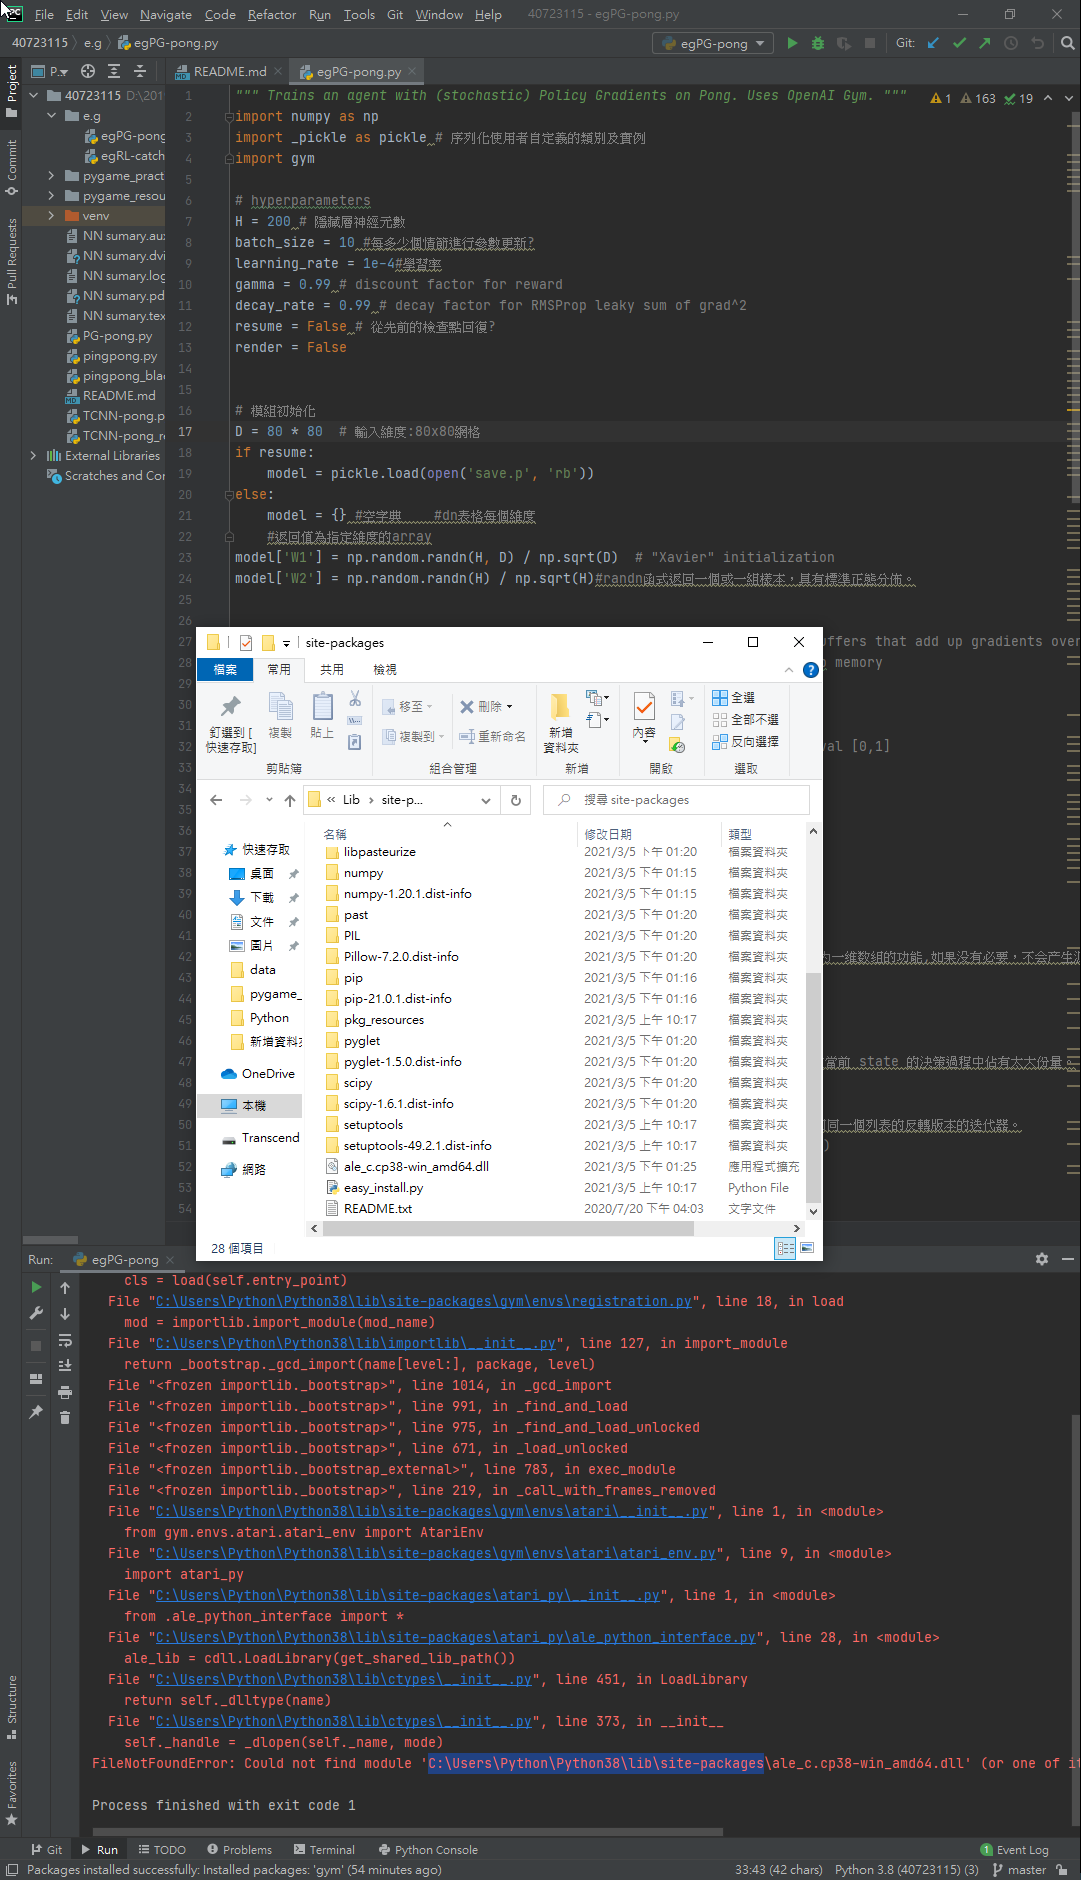
\includegraphics[width=15cm]{Q_dll}
\caption{動態連結庫錯誤}
\label{fig.動態連結庫錯誤}
\end{center}
\end{figure}

A:此問題尚未找到解決方法。\\
Q:啟用cmsimde的MathJax的功能遇到文章使用括號補充說明的內容被誤當成latex的語法轉換。\\

A:格式轉換原始定義成"("和")",所以出現誤換的問題。\\
\begin{lstlisting}[caption=MathJax 程式碼]
<script>
  MathJax = {
    tex: {inlineMath: [['$', '$'], ['\\(', '\\)']]}
  };
  </script>
  <script id="MathJax-script" 
  async src="https://cdn.jsdelivr.net/npm/mathjax@3/es5/tex-chtml.js"> 
  </script>
\end{lstlisting}

修正後將"("和")"換成"\$",就解決誤換問題
%=---------------------參考文獻----------------------=%
\newpage
\begin{center}
\addcontentsline{toc}{chapter}{參考文獻 }
\LARGE\textbf 參考文獻\\
\end{center}
\begin{flushleft}
\begin{Large}
[1]\quad https://towardsdatascience.com/derivative-of-the-sigmoid-function-536880cf918e\\

[2]\quad https://towardsdatascience.com/adam-latest-trends-in-deep-learning-optimization-6be9a291375c\\
\end{Large}
\end{flushleft}
\newpage
\begin{center}
\LARGE\textbf 作者簡介\\
\end{center}
\newpage
\begin{center}
\fontsize{0.001pt}{1pt}\selectfont .\\
\vspace{4em}
\fontsize{30pt}{30pt}\selectfont 【13】 \\
\fontsize{20pt}{40pt}\selectfont
\vspace{0.5em}
分\\
類\\
編\\
號\\
\vspace{0.5em}
\hspace{-0.5em}:\\
\vspace{0.5em}
\rotatebox[origin=cc]{270}{\sectionef\LARGE \textbf{109-4-APP-3004-1}}\\ %旋轉
\vspace{0.5em}
強\\
化\\
學\\
習\\
在\\
機\\
電\\
系\\
統\\
中\\
之\\
應\\
用\\
\vspace{2em}
一\\
一\\
零\\
級\\

\end{center}
%\newpage
%\begin{landscape}  %橫式環境
%\begin{center}
%\fontsize{0.001pt}{1pt}\selectfont .
%\vspace{70mm}
%\rotatebox[origin=cc]{90}{\LARGE 【14】}\rotatebox[origin=cc]%{180}{\LARGE 1-2-APP-8765} %旋轉
%\end{center}
%\end{landscape}
\end{document}